\documentclass[12pt,a4paper]{article}

\usepackage{graphicx}
\usepackage{subcaption}
\usepackage{booktabs}
\usepackage{multirow}
\usepackage{array}
\usepackage{float}
\usepackage{amsmath}
\usepackage{amsfonts}
\usepackage{tikz}
\usetikzlibrary{positioning, arrows.meta, matrix}
\usepackage[backend=biber, style=numeric, sorting=none]{biblatex}
\usepackage[linesnumbered,ruled,vlined]{algorithm2e}
\usepackage[hidelinks]{hyperref}
\tikzset{
  neuron/.style={circle, draw, minimum size=0.6cm, inner sep=0pt},
  layer/.style={matrix of nodes, nodes={neuron}, row sep=0.4cm, column sep=1.2cm, column 1/.style={nodes={draw=none, fill=none}}},
  connect/.style={-Stealth, thick},
}
\addbibresource{bibliography.bib} % Specify the .bib file


\setlength{\topmargin}{0.0in}
\setlength{\oddsidemargin}{0.33in}
\setlength{\textheight}{9.0in}
\setlength{\textwidth}{6.0in}
\renewcommand{\baselinestretch}{1.25}


\title{Numerical Solutions of Differential Equations using Neural Networks}

\date{Candidate Number: 1090497}

\begin{document}

\maketitle

\thispagestyle{empty}

\newpage
\setcounter{page}{1}


\section{Introduction}\label{sec: intro}
In recent years, neural networks have emerged as powerful tools in scientific computing, 
offering new ways to approximate solutions to problems traditionally addressed by numerical methods. 
While classical techniques such as finite difference, finite element, and Runge-Kutta methods remain 
foundational for solving differential equations, neural networks provide a mesh-free, 
data-driven alternative that may generalise better in certain contexts.

This report investigates the viability of neural networks for approximating solutions to 
differential equations. Rather than comparing these methods directly with classical techniques, 
we focus on evaluating their performance across a range of problem types, and on identifying 
how their effectiveness depends on architectural choices. Specifically, we consider 
their application to ordinary differential equations (ODEs), 
including initial value problems (IVPs) and boundary value problems (BVPs). We 
examine their ability to interpolate and extrapolate various types of solutions. 
As an extension, we also investigate the use of neural networks in solving selected partial 
differential equations (PDEs) using similar criteria. In each case, we analyse how performance varies 
with different network architectures and activation functions.

This report has the following structure. Section \ref{sec:preliminaries} introduces the core concepts
 of neural networks, including their architecture and training via backpropagation. It then outlines 
the specifics of using neural networks to solve differential equations, illustrating the 
methodology with a simple example. Section \ref{sec:odes} explores the use of neural networks for 
solving ODEs, dividing the discussion into IVPs and BVPs. For each, we examine a range of 
representative problems and analyse networks' ability to capture the underlying solution behaviour, and how that 
ability varies with architecture and activation function choices. Section \ref{sec:pdes}
extends the investigation to PDEs, following a similar approach. 
We test networks on a simple problem and assess how well they satisfy the relevant constraints.
Section \ref{sec:conclusion} concludes the report by summarising the findings and 
suggesting directions for further study.

\section{Preliminaries}\label{sec:preliminaries}
In this section, we outline the basic setup, components, and architecture of feedforward neural 
networks, and describe the standard approach used for training them. While multiple types of neural 
networks exist (e.g., convolutional neural networks, recurrent neural networks), we restrict our 
attention to feedforward neural networks. All references to neural networks in this report refer 
exclusively to this type.

Throughout, we adopt the following notation: vectors are denoted using lowercase bold symbols 
(e.g., $\mathbf{x}$), while matrices are written in uppercase bold (e.g., $\mathbf{W}$). We denote 
the output of the neural network as $\hat{y}$, which approximates a target function $y$.

\subsection{Neural Networks Overview and Architecture}

A feedforward neural network defines a function \( f_\theta : \mathbb{R}^n \to \mathbb{R}^m \), 
parameterised by a collection of weight matrices and bias vectors \( \theta = \{ \mathbf{W}^{(l)},
\mathbf{b}^{(l)} \}_{l=1}^L \). It is trained to approximate a target function \( y : \mathbb{R}^n \to 
\mathbb{R}^m \) using observed or synthetically generated data.

The model takes an input vector \( \mathbf{x} \in \mathbb{R}^n \) and propagates it forward through a
sequence of $L$ layers, each composed of individual units called \emph{neurons}. 

Each \emph{neuron} in a layer performs a simple two-step operation. First, it computes a weighted
sum of its inputs and adds a bias term. Then, it applies a non-linear activation function to the result.
Specifically, if a neuron with weights \( \mathbf{w}^{(l)}_i \in \mathbb{R}^{n_{l-1}} \) and bias 
\( b^{(l)}_i \in \mathbb{R} \) receives an input vector \( \mathbf{z}^{(l-1)} \in \mathbb{R}^{n_{l-1}} \), 
then its output is given by
\[
    z^{(l)}_i = \sigma\left( (\mathbf{w}^{(l)}_i)^\top \mathbf{z}^{(l-1)} + b^{(l)}_i \right),
\]
where \( \sigma: \mathbb{R} \to \mathbb{R} \) is the neuron's fixed activation function.

A layer consists of multiple such neurons, all operating in parallel on the same input vector 
\( \mathbf{z}^{(l-1)} \), each with its own weight vector and bias. The outputs from all neurons in the
layer are collected into a vector \( \mathbf{z}^{(l)} \in \mathbb{R}^{n_l} \), where \( n_l \) denotes 
the number of neurons in layer \( l \). Letting \( \mathbf{W}^{(l)} \in 
\mathbb{R}^{n_l \times n_{l-1}} \) be the matrix whose rows are the individual neuron weight vectors 
\( (\mathbf{w}^{(l)}_i)^\top \), and \( \mathbf{b}^{(l)} \in \mathbb{R}^{n_l} \) the vector of biases, 
we can express the full layer computation compactly as
\[
    \mathbf{z}^{(l)} = \sigma\left( \mathbf{W}^{(l)} \mathbf{z}^{(l-1)} + \mathbf{b}^{(l)} \right),
\]
with the activation function \( \sigma \) now applied componentwise.

The network as a whole consists of a composition of such layers. Starting from the input 
vector \( \mathbf{z}^{(0)} = \mathbf{x} \), each successive layer transforms the output of the previous
one. For a network with \( L \) layers, the computation proceeds recursively:
\[
    \mathbf{z}^{(l)} = \sigma^{(L)}\left( \mathbf{W}^{(l)} \mathbf{z}^{(l-1)} + \mathbf{b}^{(l)} 
    \right), \quad \text{for } l = 1, \dots, L-1,
\]
with the final output given by
\[
    \hat{\mathbf{y}} = f_\theta(\mathbf{x}) = \sigma^{(l)}(\mathbf{W}^{(L)} \mathbf{z}^{(L-1)} + 
    \mathbf{b}^{(L)}).
\]

The total set of network parameters \( \theta = \{ \mathbf{W}^{(l)}, \mathbf{b}^{(l)} \}_{l=1}^L \) 
are learned during training. The architecture is defined by the number of layers \( L \), the number 
of neurons \( n_l \) in each layer, and the choice of activation functions \( \sigma^{(l)} \).
The first and last layers are termed the input and output layers respectively, while intermediate 
layers are termed hidden layers. Figure \ref{fig:nn-architecture} gives an an illustrative diagram of 
a neural network architecture, with each neuron denoted by a circle, and the lines connecting each
neuron indicating an output of a single neuron being passed as an input to subsequent neurons for 
processing.

\begin{figure}[h]
    \centering
    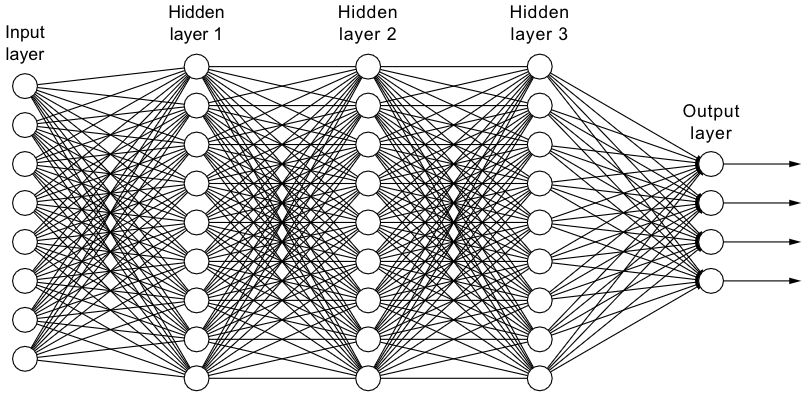
\includegraphics[width=0.7\textwidth]{graphics/neural_network_image.png}
    \caption{Illustration of a fully connected feedforward neural network with three hidden layers. 
    Each neuron computes an affine transformation of its inputs followed by a non-linear activation.}
    \label{fig:nn-architecture}
\end{figure}


Common activation functions used include:

\begin{itemize}
    \item \textbf{Hyperbolic tangent (tanh):} \quad 
    \( \sigma(x) = \tanh(x) = \dfrac{e^x - e^{-x}}{e^x + e^{-x}} \), 
    often preferred for its smoothness and differentiability.

    \item \textbf{Rectified Linear Unit (ReLU):} \quad 
    \( \sigma(x) = \max(0, x) \), 
    though not ideal when higher-order derivatives are needed.

    \item \textbf{Leaky ReLU:} \quad 
    \( \sigma(x) = 
    \begin{cases}
        x, & \text{if } x \geq 0 \\
        \alpha x, & \text{if } x < 0
    \end{cases} \), for small \( \alpha > 0 \).
    
    \item \textbf{Sinusoidal:} \quad 
    \( \sigma(x) = \sin(x) \), useful for representing oscillatory functions.
\end{itemize}

In this report we will restrict ourselves to considering these activation functions.


\subsection{Training}\label{sec:nn_training}

The parameters of a neural network — namely the weight matrices and bias vectors 
\( \theta = \{ \mathbf{W}^{(l)}, \mathbf{b}^{(l)} \}_{l=1}^L \) — are learned through a process 
called \emph{training}. The goal of training is to find a parameter set \( \theta \) such that the 
network output \( \hat{y} = f_\theta(\mathbf{x}) \) closely approximates the desired output \( y \) 
over a set of inputs \( \mathbf{x} \in \mathbb{R}^n \).

This is accomplished by defining a \emph{loss function} \( \mathcal{L}(\theta) \) that quantifies the 
discrepancy between the network predictions and the target values across a training dataset. 
In this way, training becomes a minimisation problem, where the goal is to find the parameter 
configuration $\theta^*$ that minimises the loss function $\mathcal{L}$.
When the desired outputs are continuous, a common choice is the mean squared error (MSE):
\[
    \mathcal{L}(\theta) = \frac{1}{N} \sum_{i=1}^{N} \left\| f_\theta(\mathbf{x}^{(i)}) - y^{(i)} \right\|^2,
\]
where \( \{ (\mathbf{x}^{(i)}, y^{(i)}) \}_{i=1}^N \) is the training dataset of input-output pairs.

To minimise the loss function, \( \mathcal{L}(\theta) \), a gradient-based approach 
is typically used. This requires computing the gradient of the loss with respect to all network 
parameters. This is made efficient by the \emph{backpropagation algorithm}, which systematically 
applies the chain rule of calculus to compute these derivatives by propagating error signals backward 
through the layers of the network.

Let us denote the output of layer \( l \) as \( \mathbf{z}^{(l)} \in \mathbb{R}^{n_l} \), computed via
\[
    \mathbf{z}^{(l)} = \sigma^{(l)}\left( \mathbf{a}^{(l)} \right), \quad \text{where} \quad \mathbf{a}^{(l)} = \mathbf{W}^{(l)} \mathbf{z}^{(l-1)} + \mathbf{b}^{(l)},
\]
and \( \sigma^{(l)} \) is the activation function applied componentwise.

Define the error signal at layer \( l \) as
\[
    \boldsymbol{\delta}^{(l)} := \frac{\partial \mathcal{L}}{\partial \mathbf{a}^{(l)}},
\]
which captures the sensitivity of the loss to the pre-activation input at that layer. The error at the final layer \( L \) is computed using the derivative of the loss function with respect to the network output:
\[
    \boldsymbol{\delta}^{(L)} = \nabla_{\hat{\mathbf{y}}} \mathcal{L} \odot \sigma'^{(L)}\left( \mathbf{a}^{(L)} \right),
\]
where \( \odot \) denotes elementwise (Hadamard) product and \( \sigma'^{(L)} \) is the derivative of the activation function at the final layer.

For hidden layers \( l = L-1, \dots, 1 \), the errors are computed recursively using
\[
    \boldsymbol{\delta}^{(l)} = \left( (\mathbf{W}^{(l+1)})^\top \boldsymbol{\delta}^{(l+1)} \right) \odot \sigma'^{(l)}\left( \mathbf{a}^{(l)} \right).
\]

Once the error signals are computed for each layer, the gradients of the loss with respect to the weights and biases are given by
\[
    \frac{\partial \mathcal{L}}{\partial \mathbf{W}^{(l)}} = \boldsymbol{\delta}^{(l)} (\mathbf{z}^{(l-1)})^\top, \quad
    \frac{\partial \mathcal{L}}{\partial \mathbf{b}^{(l)}} = \boldsymbol{\delta}^{(l)}.
\]

These gradients are then used in an optimisation routine (e.g., stochastic gradient descent) to update the parameters:
\[
    \mathbf{W}^{(l)} \leftarrow \mathbf{W}^{(l)} - \eta \frac{\partial \mathcal{L}}{\partial \mathbf{W}^{(l)}}, \quad
    \mathbf{b}^{(l)} \leftarrow \mathbf{b}^{(l)} - \eta \frac{\partial \mathcal{L}}{\partial \mathbf{b}^{(l)}},
\]
where \( \eta > 0 \) is the learning rate.

This process is repeated iteratively over the training data until convergence to a (local) minimum of the loss function. In practice, more advanced optimisers such as Adam or RMSProp are often used, which adaptively adjust the learning rate based on estimates of past gradients.

\section{Ordinary Differential Equations}\label{sec:odes}
Having outlined the methodology for using neural networks to solve differential equations, in this 
section, we begin a more systematic investigation of their performance across a range of ODE problems.
This section is divided into two main parts: initial value problems (IVPs) and boundary value problems
(BVPs). In each case, we examine the extent to which neural networks can learn accurate solutions 
and how their performance is affected by architectural choices.

In the IVP setting, we consider three representative classes of problems: exponential decay,
periodic solutions, and solutions containing a singularity. These problems allow us to assess 
both interpolation accuracy and a network's ability to extrapolate beyond the training domain.

For BVPs, our focus will remain on evaluating the quality of the approximation within the 
prescribed domain. Since boundary conditions are enforced at fixed endpoints, extrapolation 
beyond the interval is not typically meaningful. Instead, we investigate how the network adapts
to constraints at both boundaries, and how well it captures internal behaviour with different
choices of architecture and optimisation.

To systematically explore the influence of key design parameters, for each problem, we will vary: 
the number of neurons per hidden layer, the number of hidden layers and the choice of activation 
function. These experiments will serve to assess neural networks' ability to solve differential 
equation problems, along with understanding how this ability varies with architectural choices. 
We do not consider networks with different numbers of neurons in each layer, and we use the MSE
loss function for all models. We choose between the $\tanh$ and ReLU activation functions,
these being two of the most common activation functions chosen \cite{goodfellow2016deep}, 
and use the same activation functions in all networks, as is standard practice \cite{goodfellow2016deep}.

We deliberately restrict our investigation to variations in network architecture and activation 
functions, holding other hyperparameters fixed (such as the learning rate, optimiser type, and 
penalty parameters for enforcing boundary conditions). This choice simplifies the analysis and 
enables a clearer interpretation of the results by isolating the effects of architectural design. 
Our primary interest lies in the representational capability of neural networks — that is, how 
well different architectures can approximate solutions once trained — rather than in training 
efficiency. Provided that convergence is achieved, changes to hyperparameters like the learning 
rate or penalty weight primarily influence the speed or stability of training and not the final quality 
of the fit. To this end, we use the Adam optimiser, which is widely regarded as robust to 
hyperparameter settings such as the learning rate and penalty weight (\cite{goodfellow2016deep},
Section 8.5.4). To ensure fairness and comparability, all models were trained for the same 
number of epochs (typically 2500) with 100 training points in the domain, plus the 
boundary/initial value points. A learning rate of $\alpha = 0.001$ and penalty weight 
$\gamma = 100$ were used. All 
models were implemented in Python using the PyTorch library \cite{paszke2017automatic}.


\subsection{Initial Value Problems}\label{sec:IVPs}

\subsubsection{Exponential Decay}

We begin our analysis with a simple initial value problem whose solution exhibits exponential decay:
\[
\begin{aligned}
    y'(x) &= -y(x), \\
    y(0) &= 1.
\end{aligned}
\]
The exact solution is \( y(x) = e^{-x} \), a smooth and monotonic function defined on the entire real
line. This problem provides a natural baseline for assessing the ability of neural networks to 
approximate well-behaved solutions and to generalise beyond the training interval.

We train a series of feedforward neural networks on this problem using the architectural variation 
strategy described previously. Results for 
both \(\tanh\) and ReLU activation functions are shown in Figure~\ref{fig:expdecay_sidebyside}, 
including error heatmaps and examples of the best and worst performing networks under each 
activation function.

\begin{figure}[htbp]
    \centering
    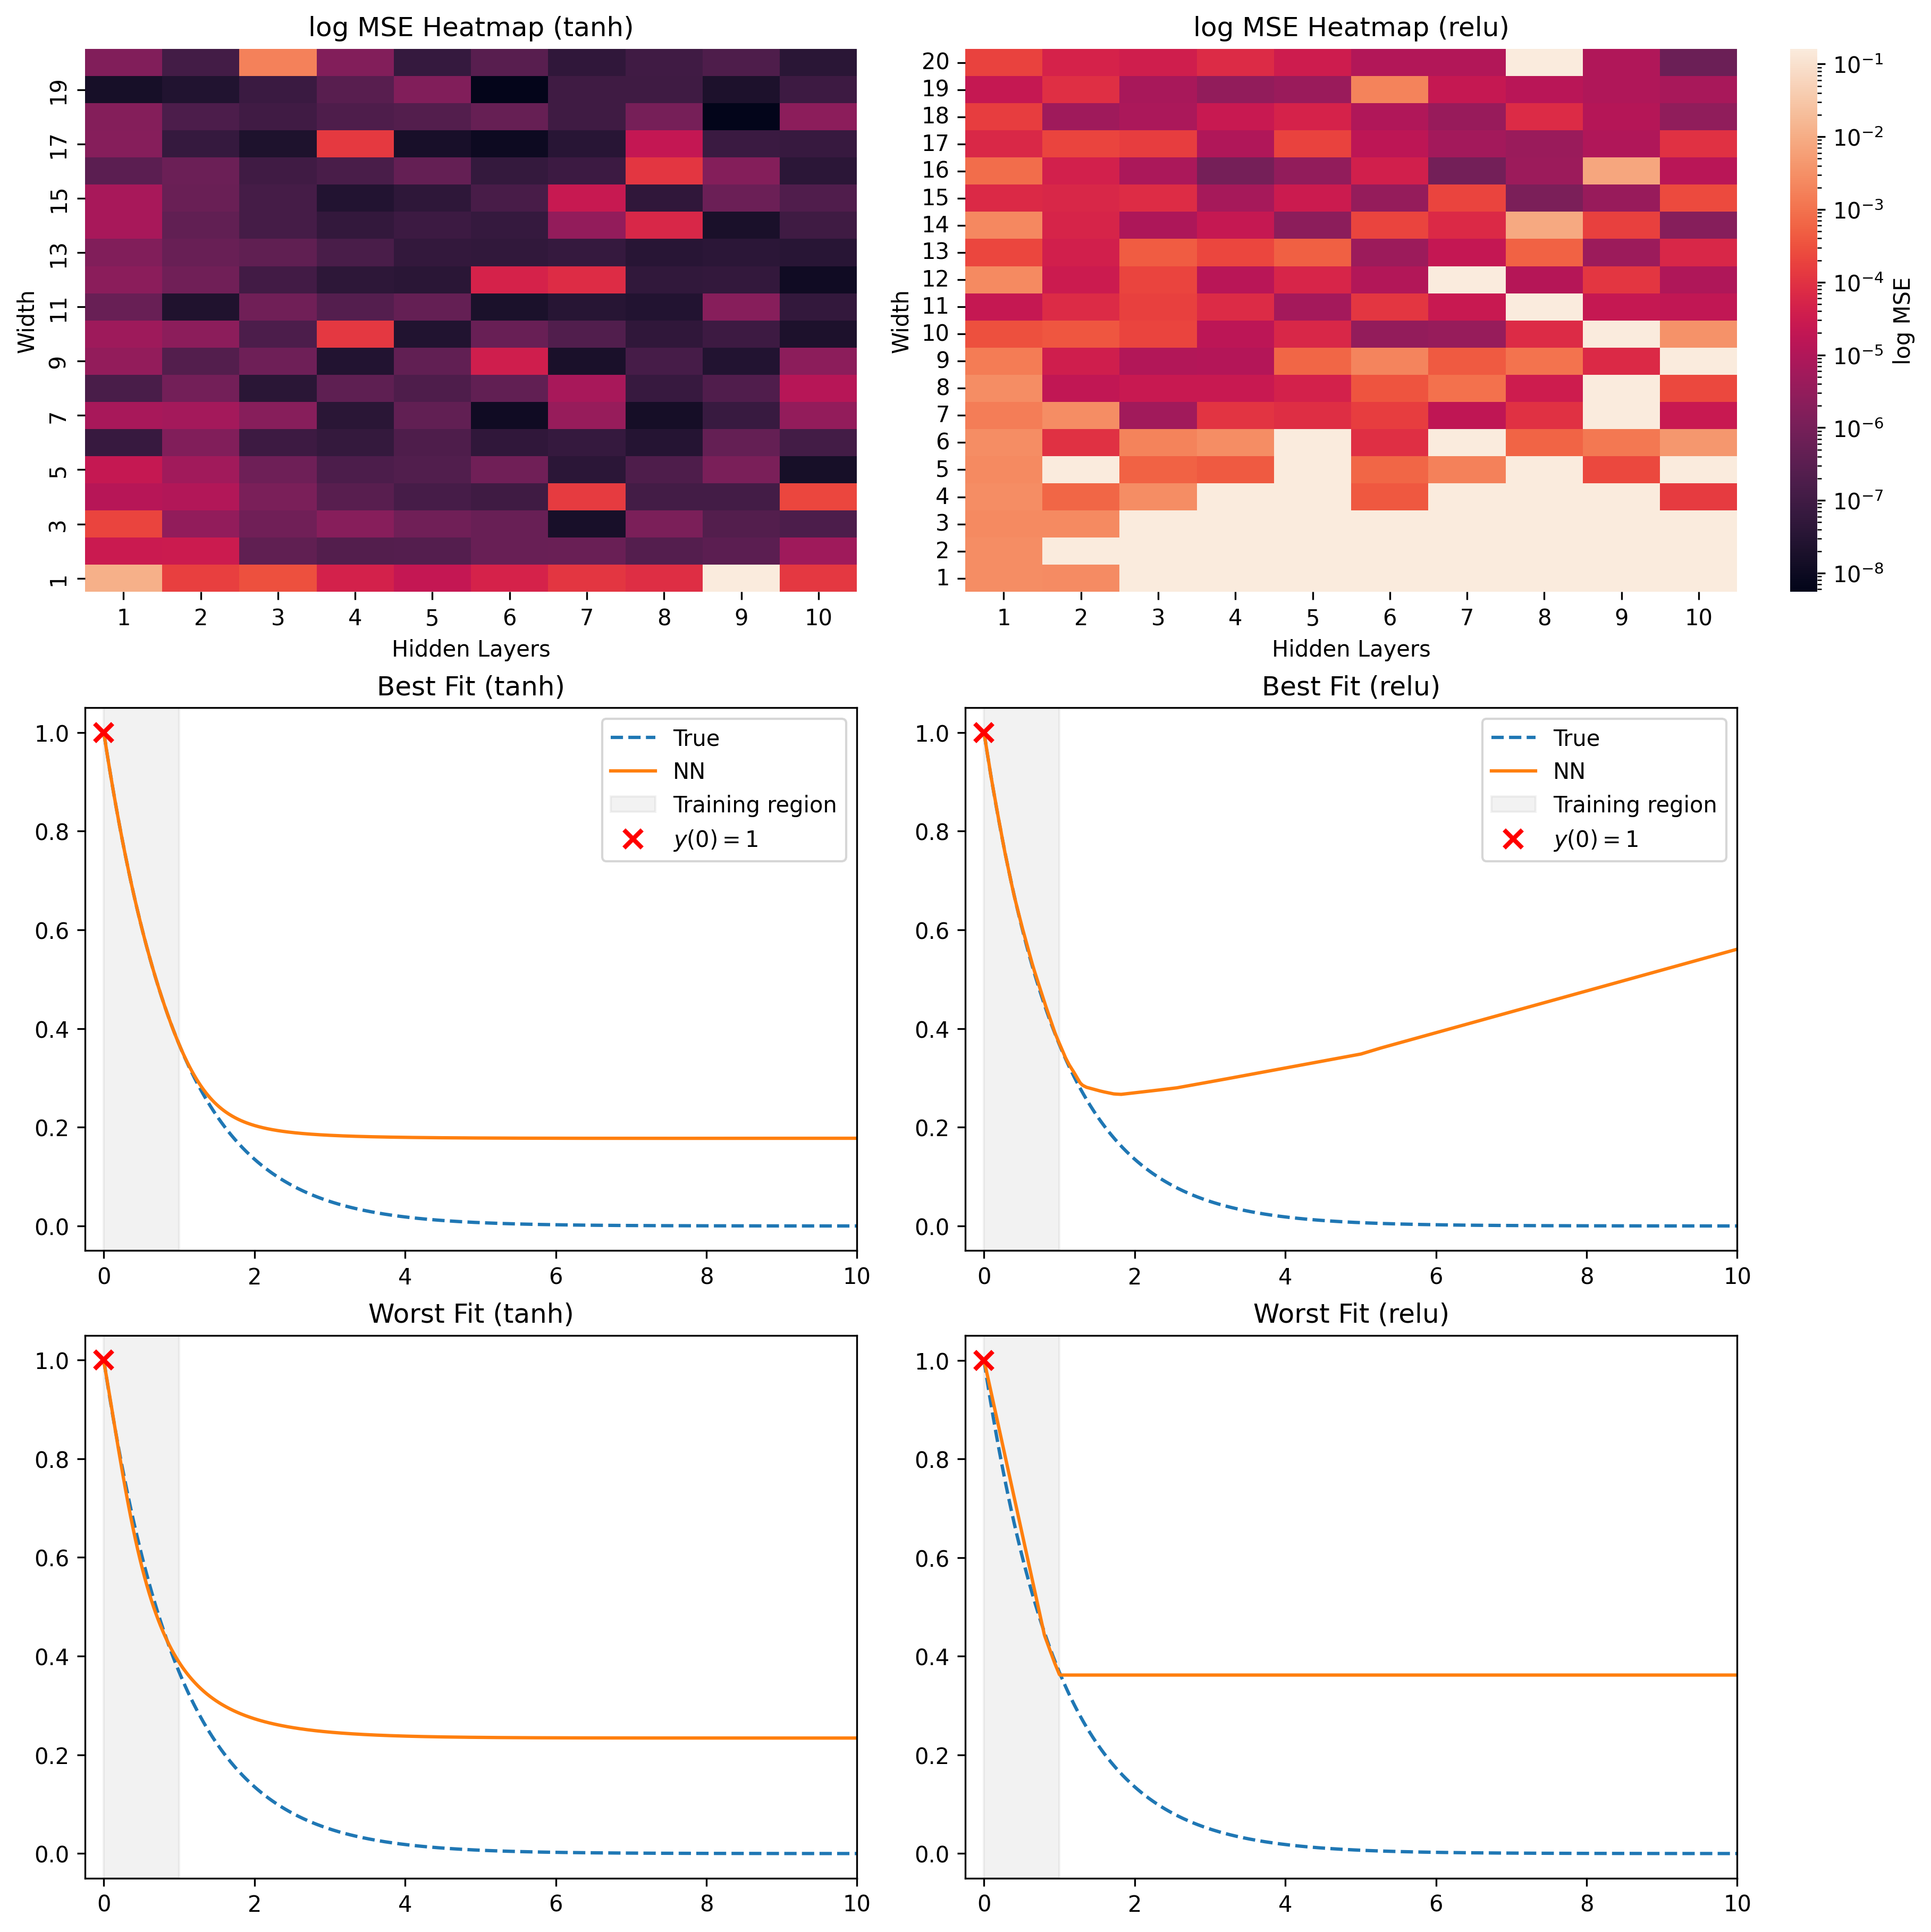
\includegraphics[width=\textwidth]{graphics/ivp_exponential_combined.png}
    \caption{Comparison of architectural performance for the exponential decay problem using two 
    activation functions. Each column shows the MSE heatmap with a log error scale,
    the best network fit, and the worst network fit.}
    \label{fig:expdecay_sidebyside}
\end{figure}


The heatmaps in Figure~\ref{fig:expdecay_sidebyside} reveal several consistent trends. For 
both activation functions, increasing the number of neurons per layer leads to improved 
accuracy for a fixed number of layers. In contrast, increasing depth alone did not guarantee better 
performance, particularly when layers are narrow. The best-performing configurations are found with 
moderately deep networks (4--8 layers) and wider layers (10--20 neurons), though the overall 
sensitivity to architecture is relatively mild, likely due to the simplicity of the target 
function. More striking differences emerge in extrapolation. The ReLU-based networks fail to 
capture the exponential decay beyond the training domain, typically reverting to a linear 
trajectory. By contrast, the networks trained with \(\tanh\) not only interpolate more accurately 
even in the worst case, but also exhibit qualitatively correct exponential behaviour when extrapolated 
to \(x = 10\). Finally, we observe in our heatmap that the error for most neural network architectures 
using the $\tanh$ activation function has lower MSE than those using the ReLu function, regardless 
of architecture, suggesting that the choice of activation function is a key determinant of quality of 
fit.



\subsubsection{Periodic Solution}

We now consider an initial value problem whose solution is periodic:
\[
\begin{aligned}
    y'(x) &= \cos x, \\
    y(0) &= 0.
\end{aligned}
\]
The exact solution is \( y(x) = \sin x \), which is smooth, bounded, and periodic with period \( 2\pi \).  
This problem allows us to evaluate the capacity of neural networks to approximate oscillatory behaviour
across a wide domain, and to generalise that behaviour beyond the domain.  

We perform the same analysis as in the previous section, first analysing how the error varies
for different architectures, and then examining the best solutions (we exclude the worst 
cases from now, as these were purely for comparison in the preceding section), shown in Figure 
\ref{fig:ivp_periodic_sidebyside}.

\begin{figure}[h]
    \centering
    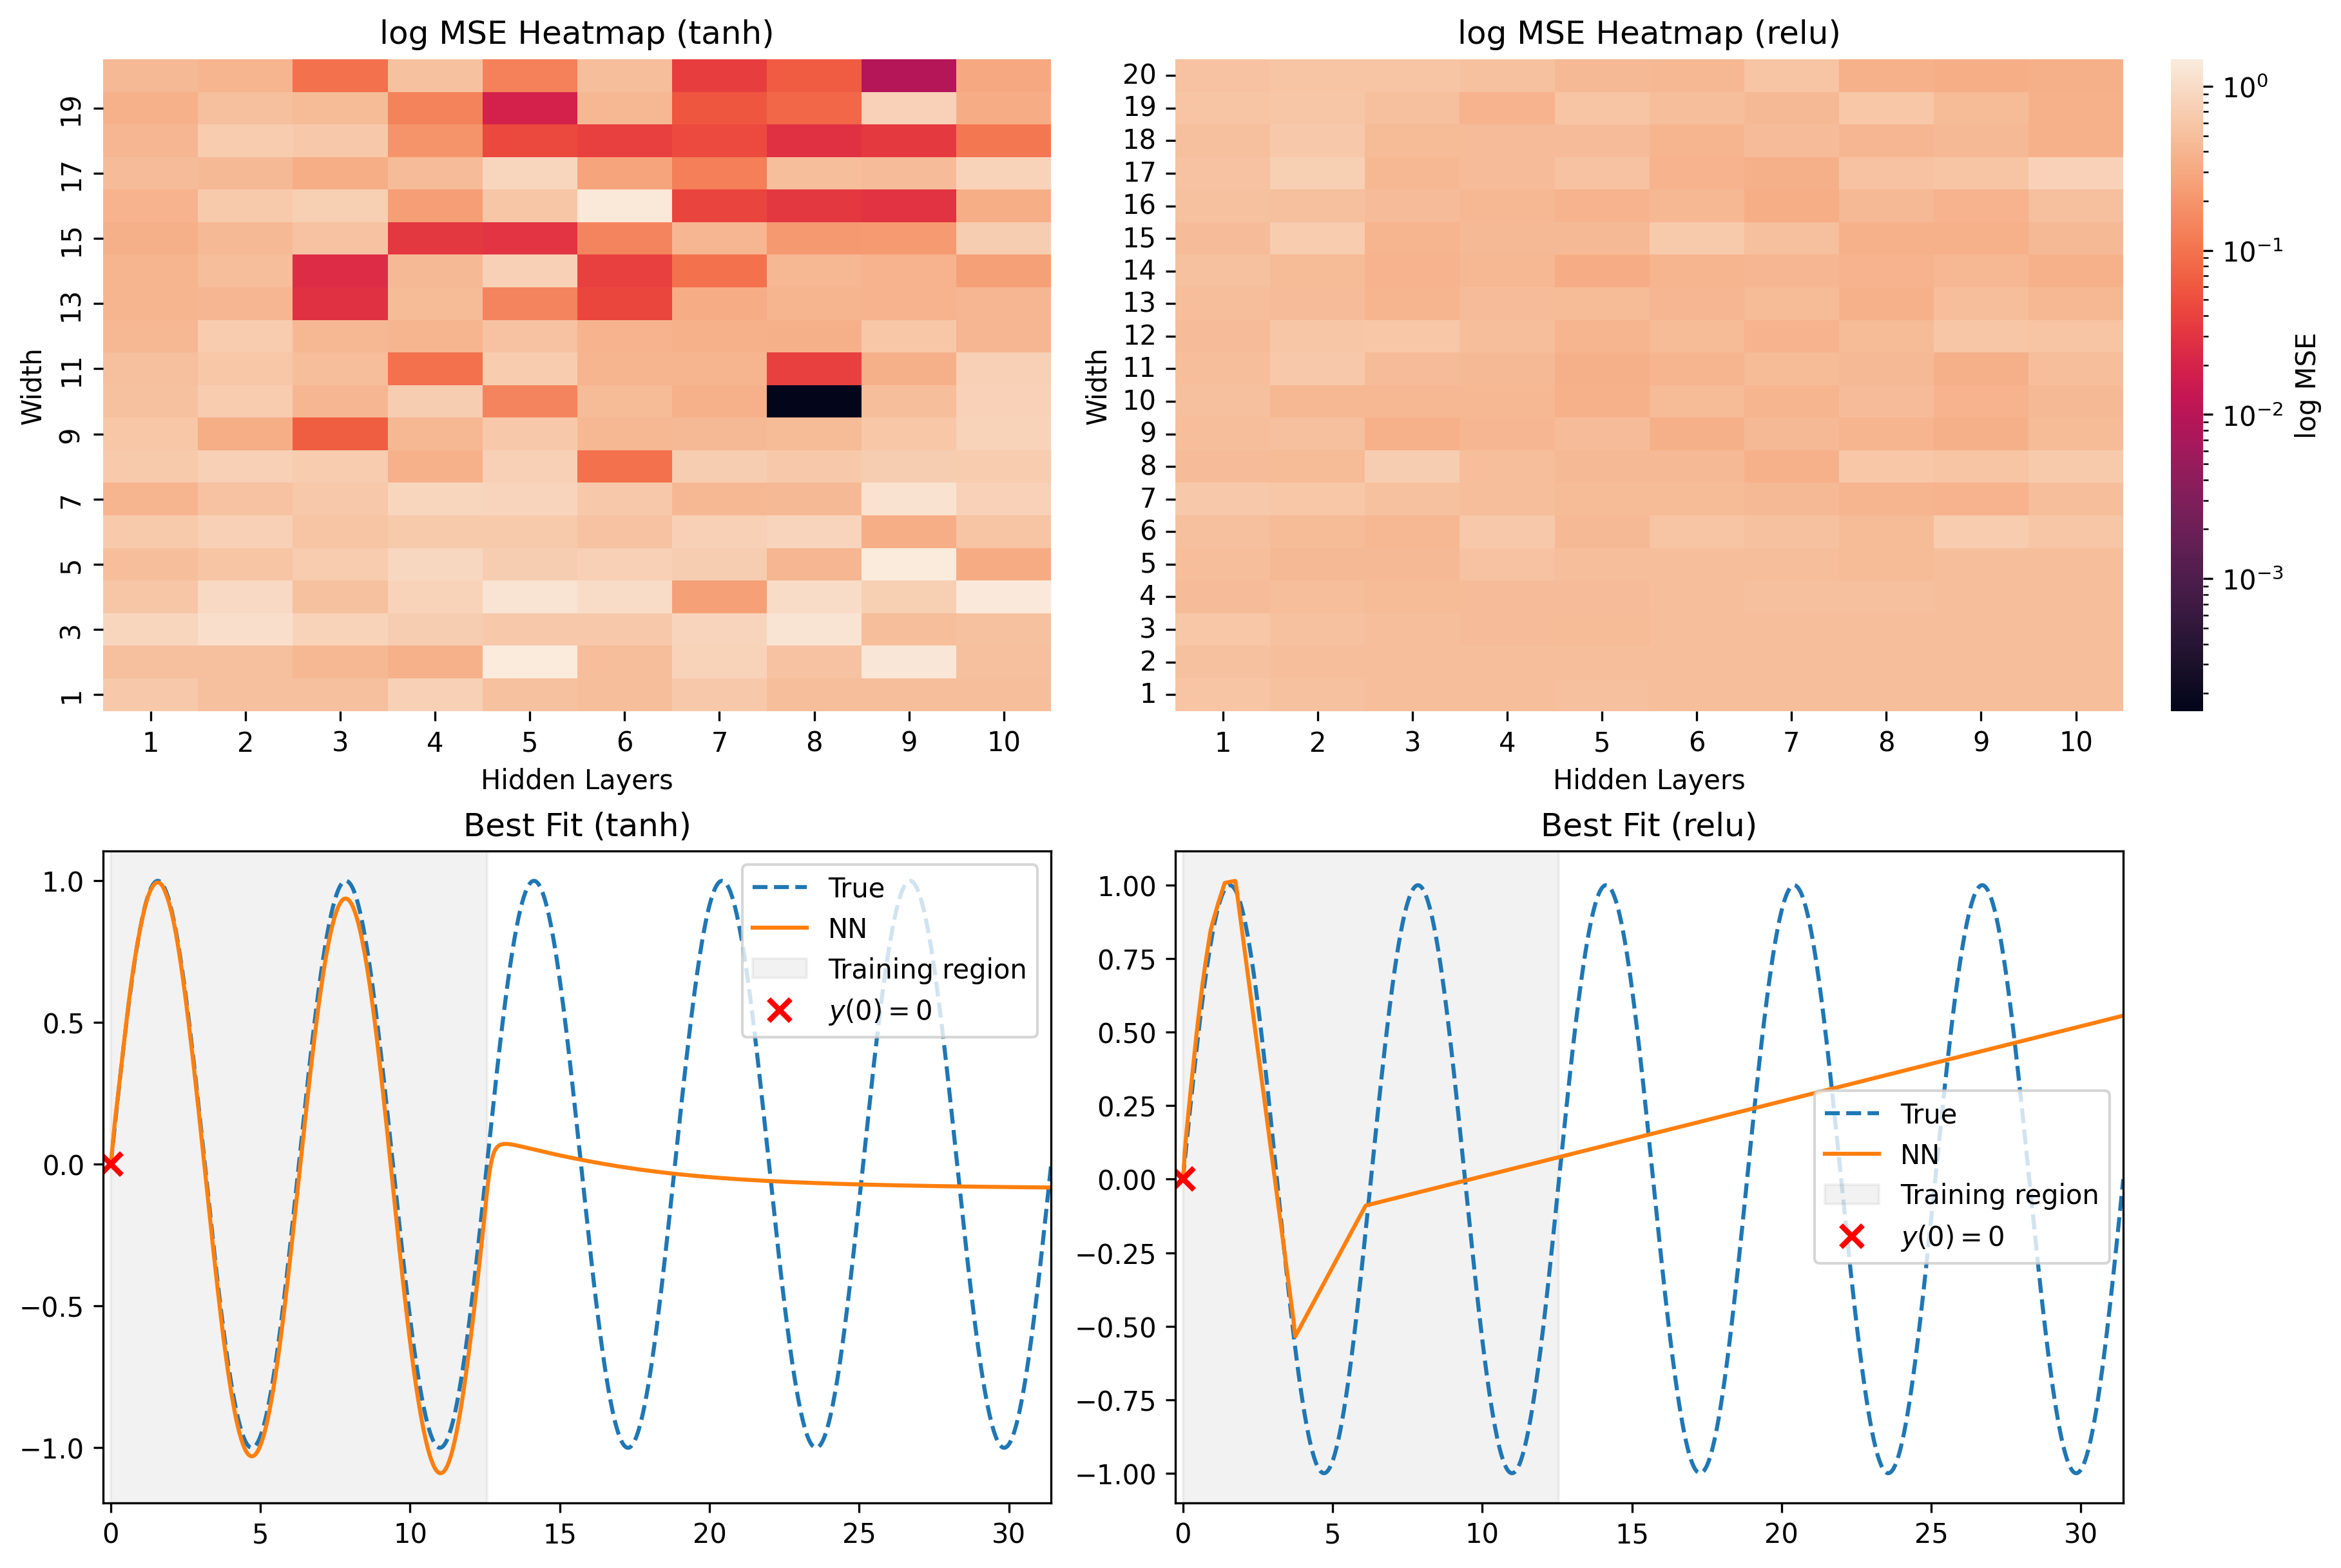
\includegraphics[width=\textwidth]{graphics/ivp_periodic_combined.png}
    \caption{Comparison of architectural performance for the oscillatory problem using two 
    activation functions. Each column shows the MSE heatmap with a log error scale,
    the best network fit for each activation function.}
    \label{fig:ivp_periodic_sidebyside}
\end{figure}

We observe that the choice of activation function has a significant impact on the network's 
ability to approximate this solution, the ReLU networks seeing negligible improvements 
in fit as the architecture was varied, and the \(\tanh\) activation function yielding 
noticeably better fits than ReLU. This is intuitive: \(\tanh\) is smooth and nonlinear, 
sharing important qualitative features with \(\sin(x)\), while ReLU is only piecewise linear 
and lacks curvature. As such, we would expect ReLU networks to require substantially greater 
depth and width to match the expressivity of a \(\tanh\)-based network. 
Both activations struggle to extrapolate periodicity beyond the training domain.
The predicted solutions flatten outside the interval, rather than 
propagating sinusoidal behaviour.


\subsubsection{Singular Solution}

We now turn to an initial value problem whose solution contains a singularity:
\[
\begin{aligned}
    y'(x) &= y(x)^2, \\
    y(0) &= 1, \\
    y(1.05) &= -20
\end{aligned}
\]
The exact solution is \( y(x) = \frac{1}{1 - x} \), which becomes singular at \( x = 1 \). This 
problem is useful for testing the ability of neural networks to approximate rapidly varying functions 
and to capture solution blow-up within a finite domain.

To mitigate instability near the singularity, we train two separate networks: one on the interval 
\([0, 0.95]\) using the initial condition \( y(0) = 1 \), and one on the interval \([1.05, 2.0] \) 
using the condition \( y(1.05) = -20 \). This approach allows us to evaluate how 
well neural networks can approximate the solution on either side of the singularity without 
numerical breakdown. Results are shown in Figure \ref{fig:ivp_singular_sidebyside}.

\begin{figure}[h]
    \centering
    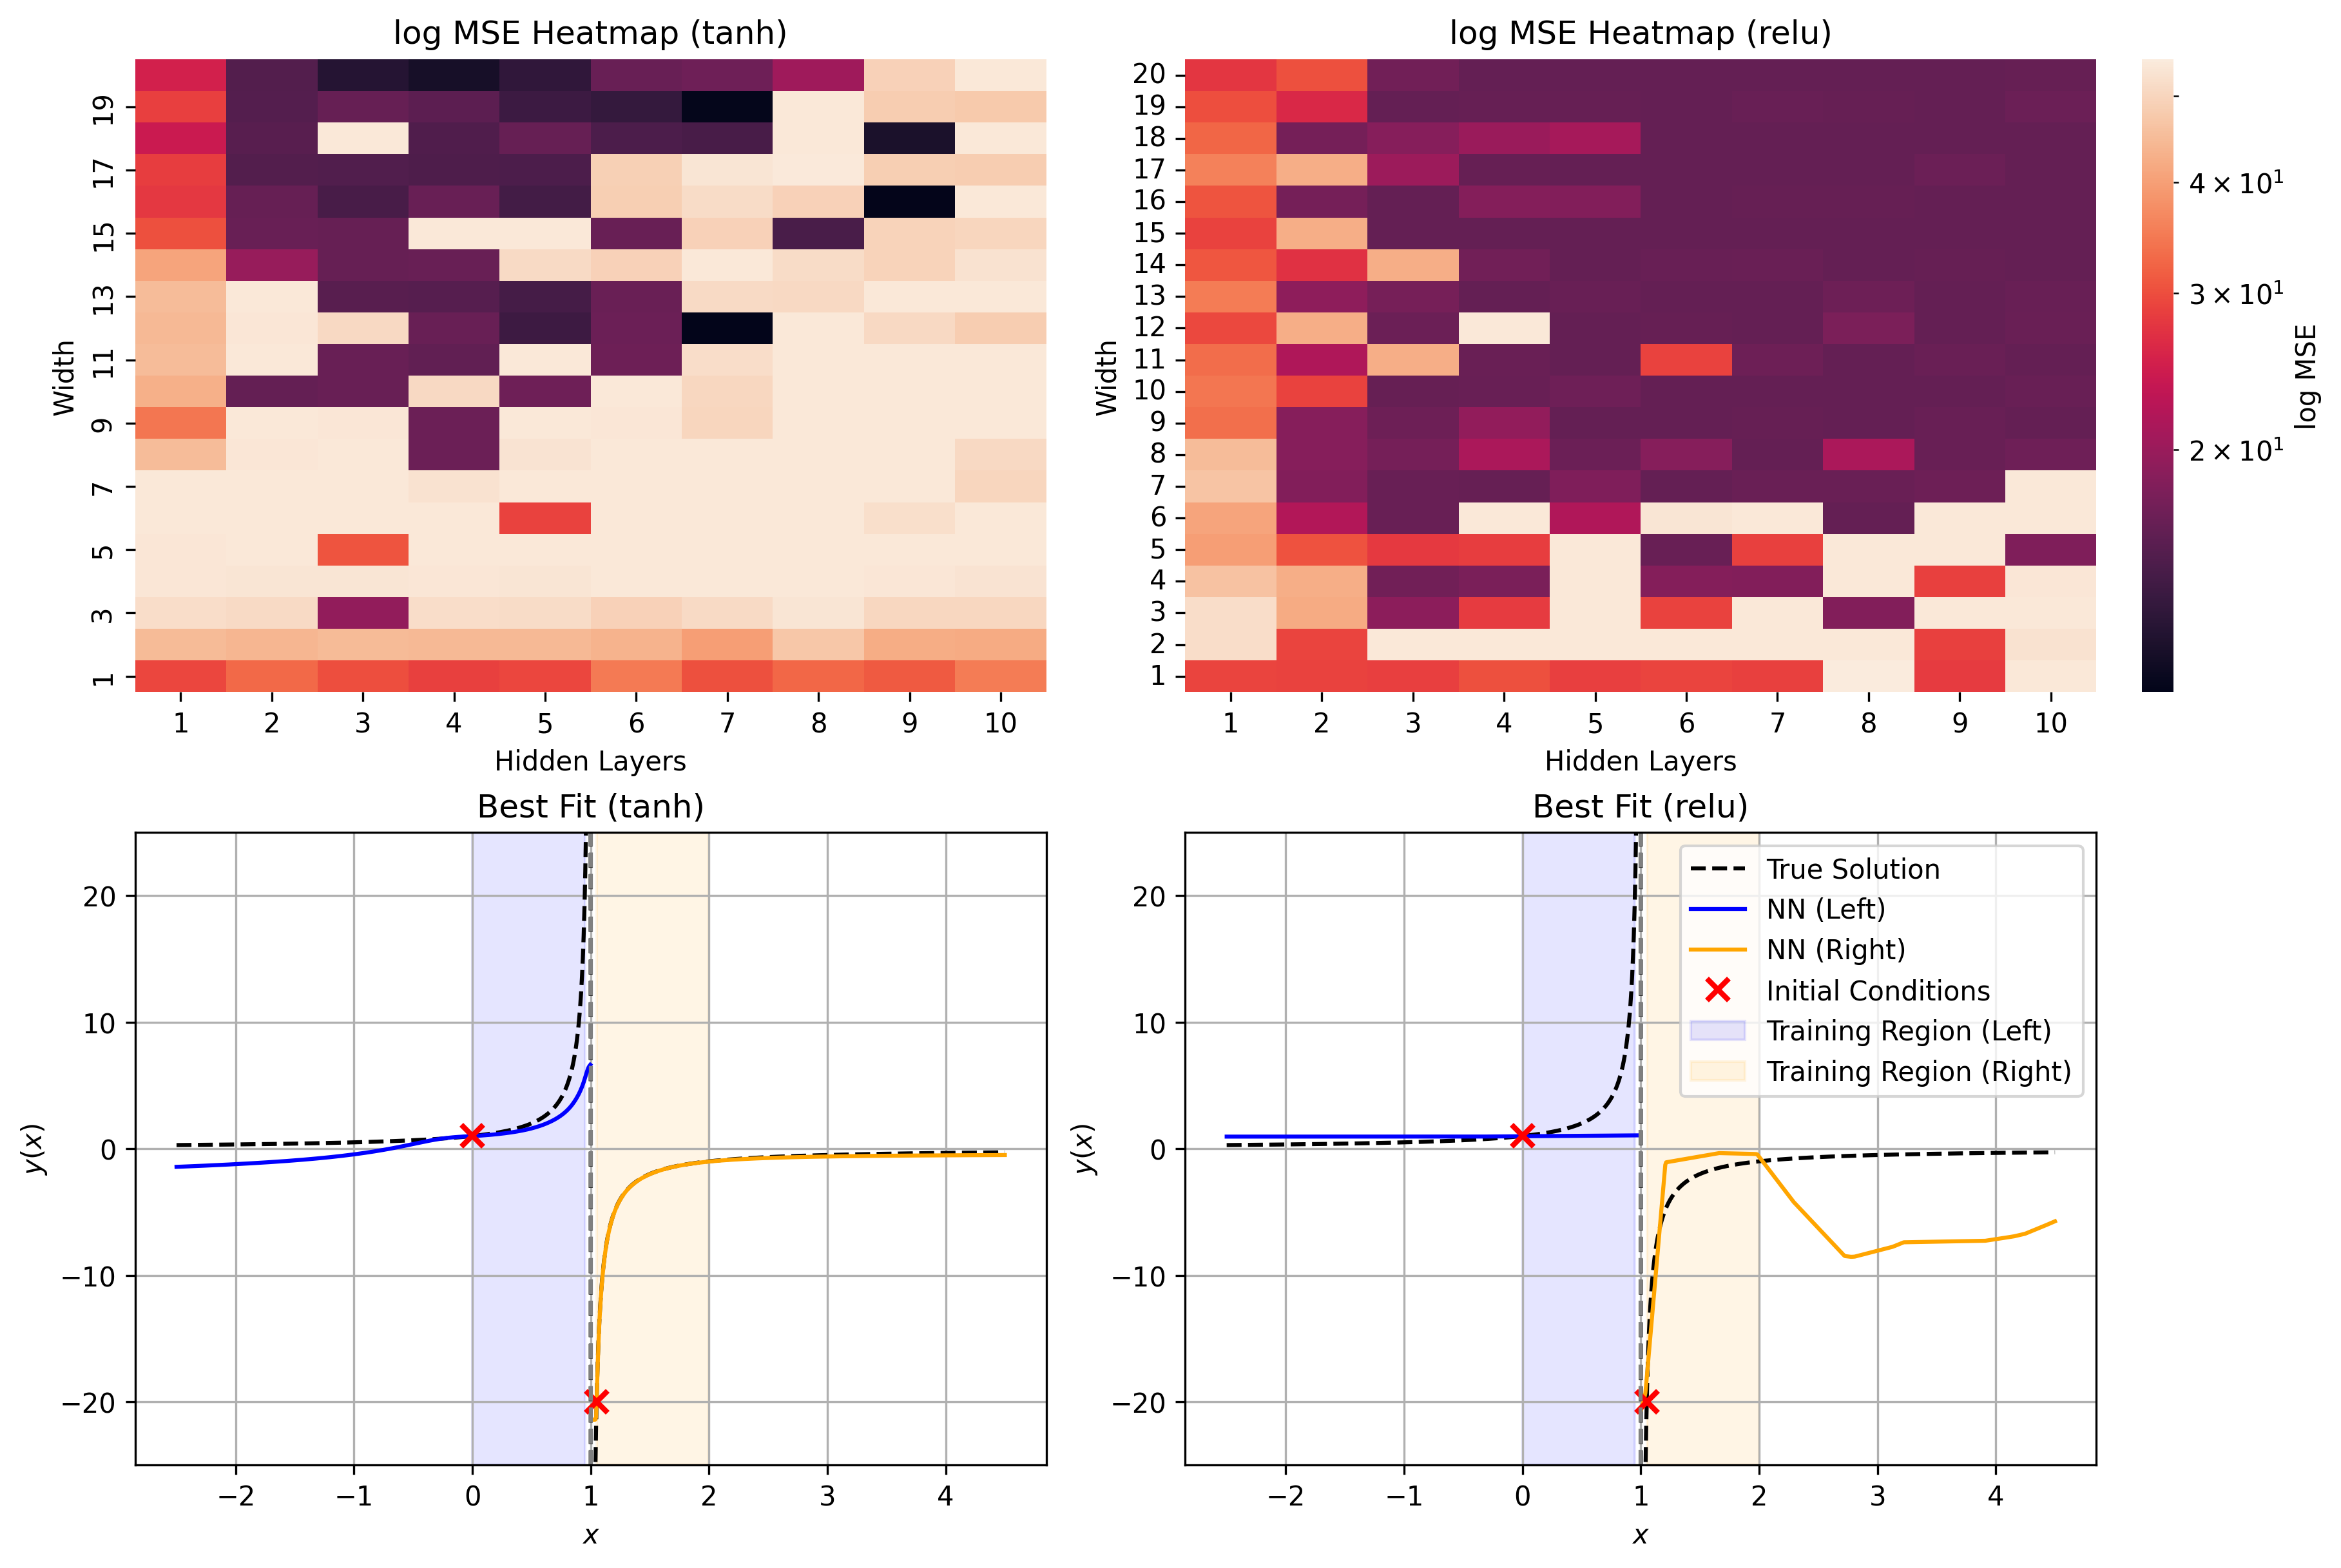
\includegraphics[width=\textwidth]{graphics/ivp_singularity_combined.png}
    \caption{Comparison of architectural performance for the singular solution problem using two 
    activation functions. Each column shows the MSE heatmap with a log error scale,
    the best network fit, and the worst network fit.}
    \label{fig:ivp_singular_sidebyside}
\end{figure}

Figure~\ref{fig:ivp_singular_sidebyside} shows that while the ReLU activation function yields 
lower MSE across a broader range of architectures, the \(\tanh\) activation achieves significantly
better fits for select configurations. Notably, networks using \(\tanh\) require at least 7 hidden 
layers to perform well, with accuracy dropping sharply for deeper architectures beyond 8 layers. 
An interesting pattern emerges with respect to width: networks with only one neuron per layer often 
outperform those with 2-3 neurons, suggesting that minimal width can sometimes aid in learning steep 
gradients near singularities. In terms of qualitative behaviour, the best \(\tanh\) network closely 
tracks the exact solution on the right side of the singularity and extrapolates smoothly beyond the 
training region, converging to a nearly linear continuation, while also beginning to capture the shape
on the left side. In contrast, the ReLU network produces jagged, piecewise responses outside the 
training domain, failing to capture the smooth decay, and completely failing 
to capture the structure on the left of the singularity.



\subsection{Boundary Value Problems}\label{sec:BVPs}


We now consider boundary value problems (BVPs), where the solution is defined by a 
differential equation along with prescribed values at the boundaries of a fixed domain. Unlike 
initial value problems, BVPs specify constraints at multiple points—typically at the endpoints of 
an interval—and the solution must satisfy the differential equation throughout the domain while 
adhering to these boundary conditions.

In this section, we investigate how well neural networks can approximate solutions to BVPs using 
the same methodology outlined for IVPs. However, since BVPs are defined strictly on a bounded 
interval, we do not consider extrapolation performance here. Instead, we focus on how accurately 
the networks capture the solution within the specified domain.

We consider two BVPs:
\begin{itemize}
    \item A smooth Poisson-type problem, with known analytic solution $y(x)=sin(\pi x)$, 
    serving as a baseline. 
    \item A piecewise forcing problem with a discontinuous right-hand side, used to examine network
     behaviour under more challenging conditions. 
\end{itemize}




\subsubsection{Poisson Problem}

We begin with a classical boundary value problem from mathematical physics:
\[
\begin{aligned}
    -y''(x) &= \pi^2 \sin(\pi x), \quad x \in (0, 1), \\
    y(0) &= 0, \\
    y(1) &= 0.
\end{aligned}
\]
This has the exact solution \( y(x) = \sin(\pi x) \), which is smooth, bounded, and vanishes at both 
endpoints. The problem provides a simple setting to evaluate how well neural networks approximate 
solutions to second-order differential equations with smooth forcing and well-defined boundary 
conditions, and how those approximations vary with architecture.

As in the IVP analysis, we assess the effect of architectural variation on solution accuracy.
For each combination of depth, width, and activation function, we compute the MSE across the domain,
and visualise the results using heatmaps and the best fits, shown in 
Figure~\ref{fig:bvp_poisson_sidebyside}.

\begin{figure}[h]
    \centering
    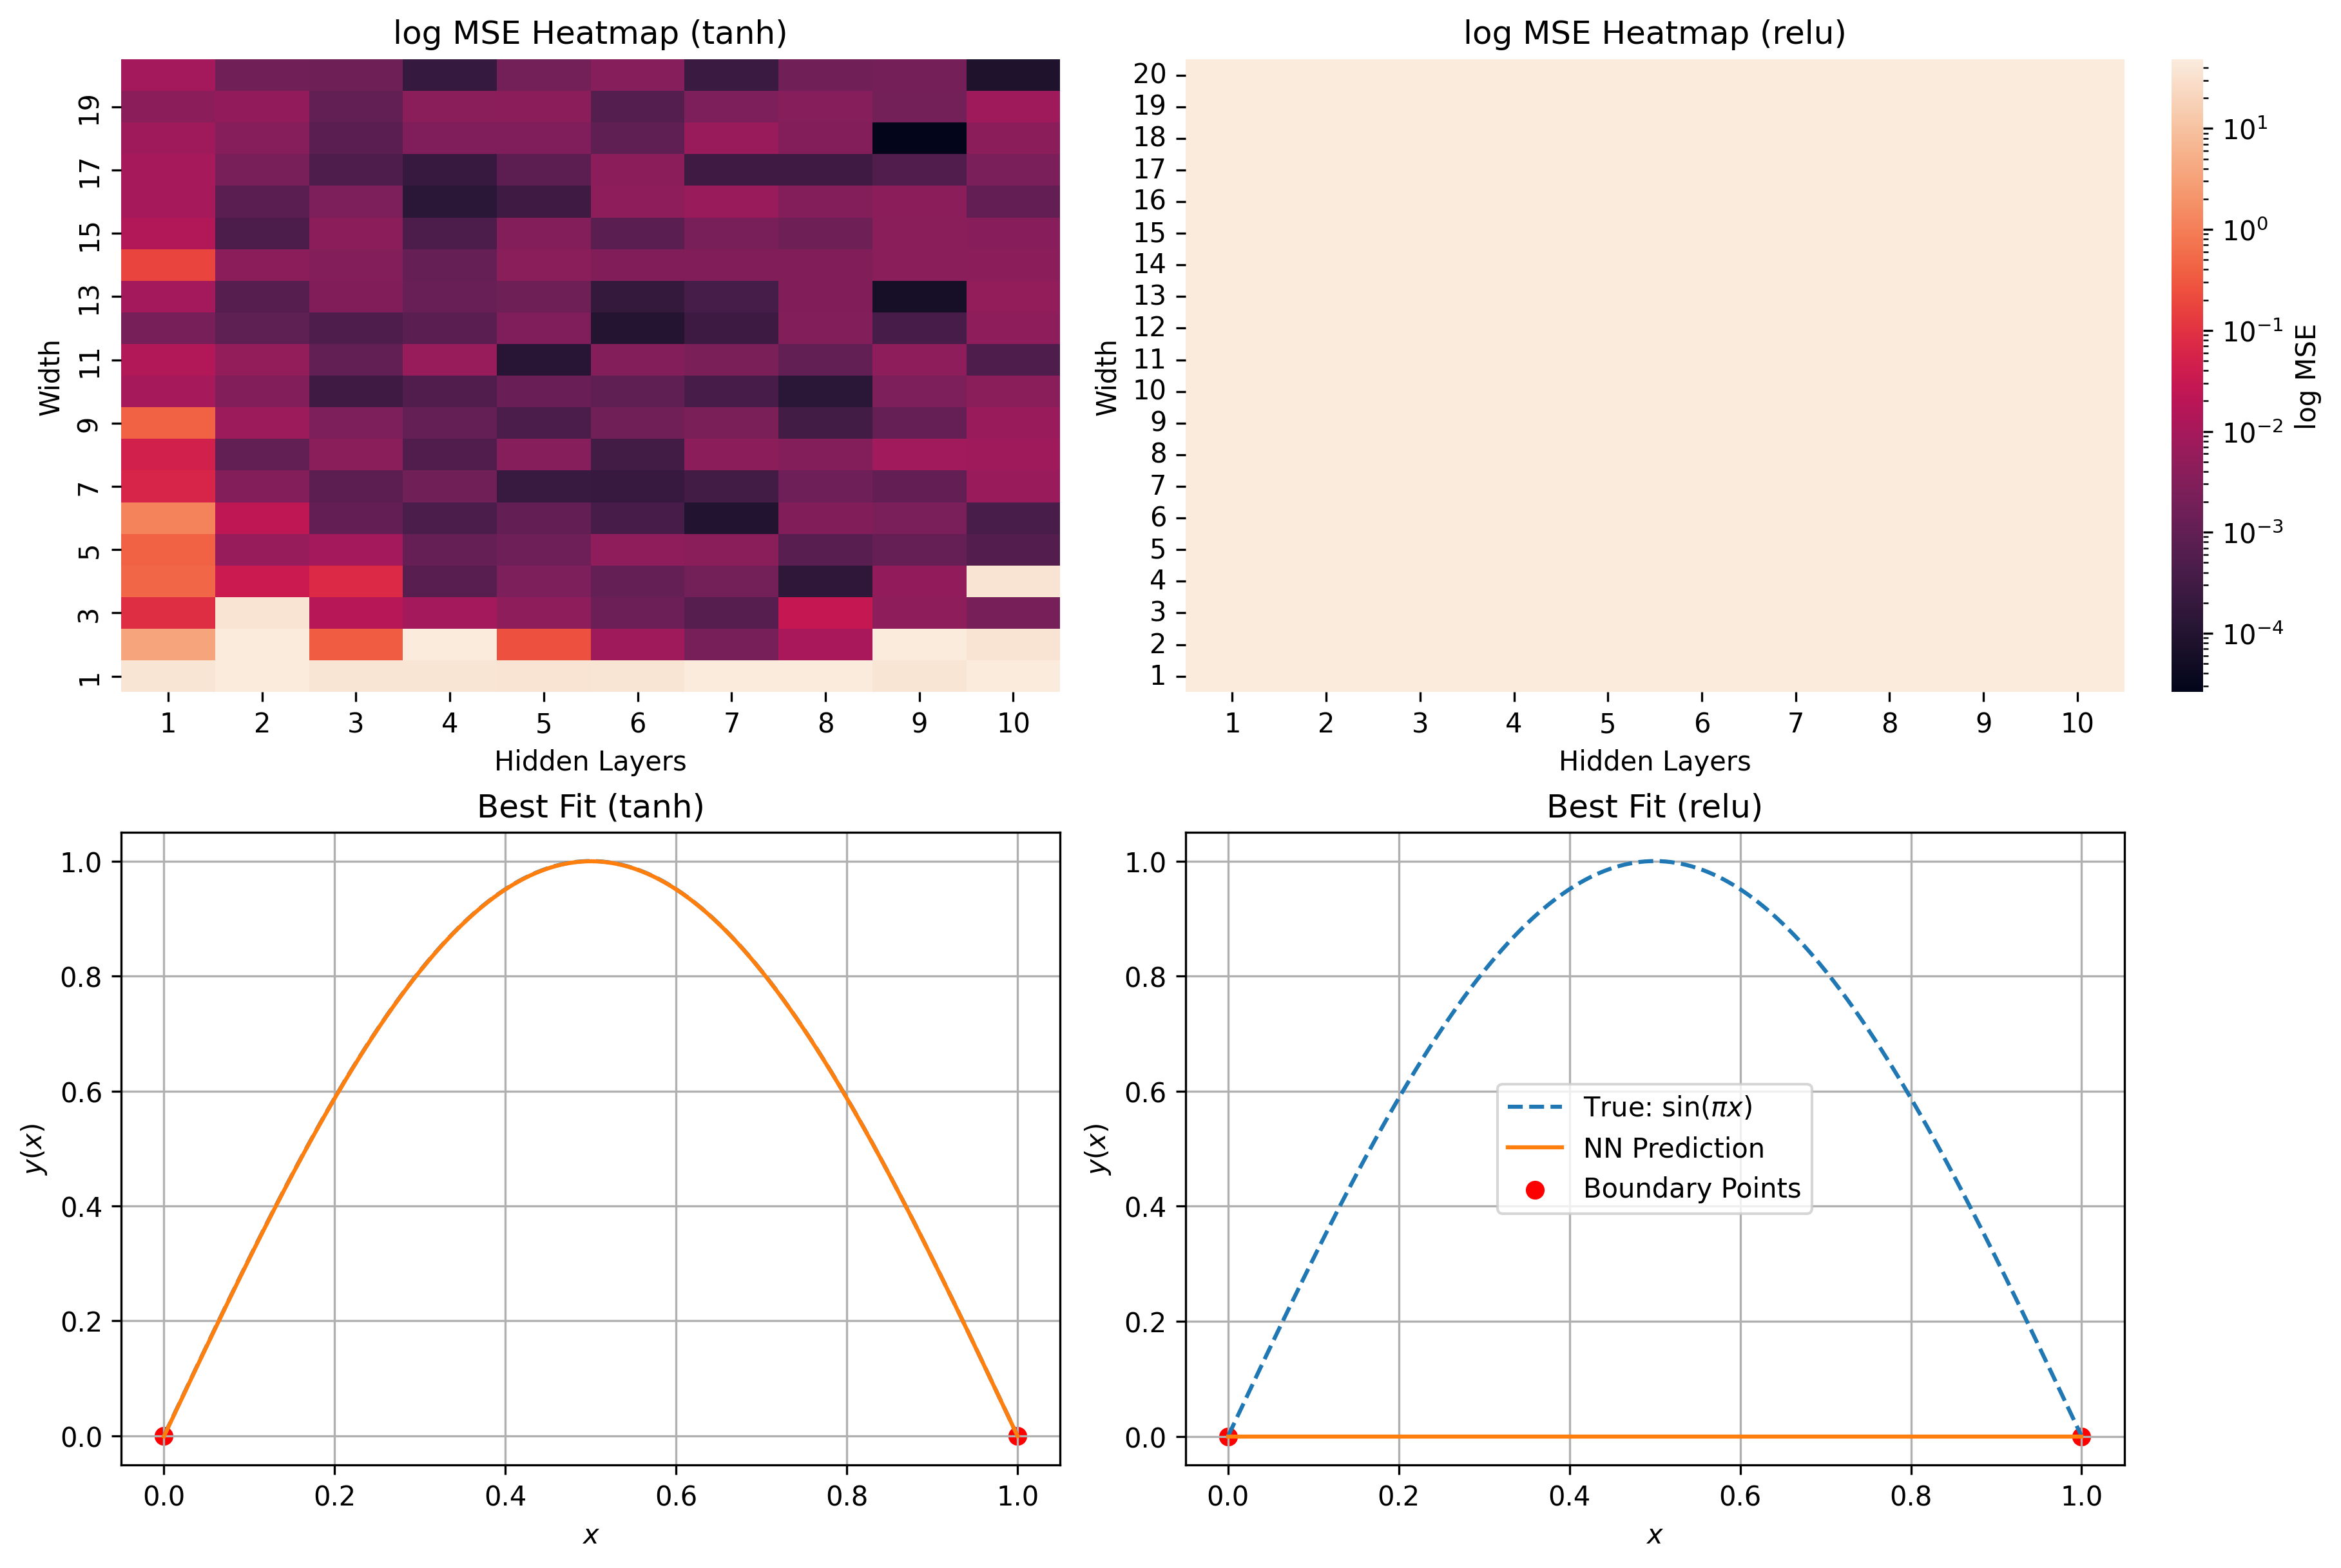
\includegraphics[width=\textwidth]{graphics/bvp_poisson_combined.png}
    \caption{Comparison of architectural performance for the Poisson BVP using two 
    activation functions. Each column shows the MSE heatmap with a log error scale,
    the best network fit, and the worst network fit.}
    \label{fig:bvp_poisson_sidebyside}
\end{figure}

The ReLU activation function exhibits a clear inability to capture the curvature of the solution 
in this problem. Across all tested architectures, it appears to reduce error primarily by satisfying
the boundary conditions, rather than accurately fitting the interior solution. In contrast, 
the $\tanh$ activation function consistently achieves an excellent approximation, with 
performance improving steadily as both depth and width are increased. This result is 
consistent with earlier observations, where $\tanh$ proved particularly well-suited to 
approximating sinusoidal solutions over the training domain.

\subsubsection{Piecewise Forcing}

We now consider a boundary value problem with a discontinuous right-hand side:
\[
\begin{aligned}
    y''(x) &= 
    \begin{cases}
        -1, & 0 \leq x < 0.5, \\
        +1, & 0.5 \leq x \leq 1,
    \end{cases} \\
    y(0) &= 0, \\
    y(1) &= 0.
\end{aligned}
\]
The exact solution is piecewise quadratic, continuous, and satisfies the boundary conditions. 
However, the discontinuity in the forcing term induces a derivative jump at \( x = 0.5 \), 
making this a challenging test case for smooth neural network approximators.

This example allows us to assess how well neural networks can adapt to discontinuous dynamics
in the governing equation. As before, we systematically vary network architecture and activation 
function, compute the corresponding approximation error, and visualise representative results.
The best-fitting solutions are summarised in Figure~\ref{fig:bvp_piecewise_sidebyside}.

\begin{figure}[h]
    \centering
    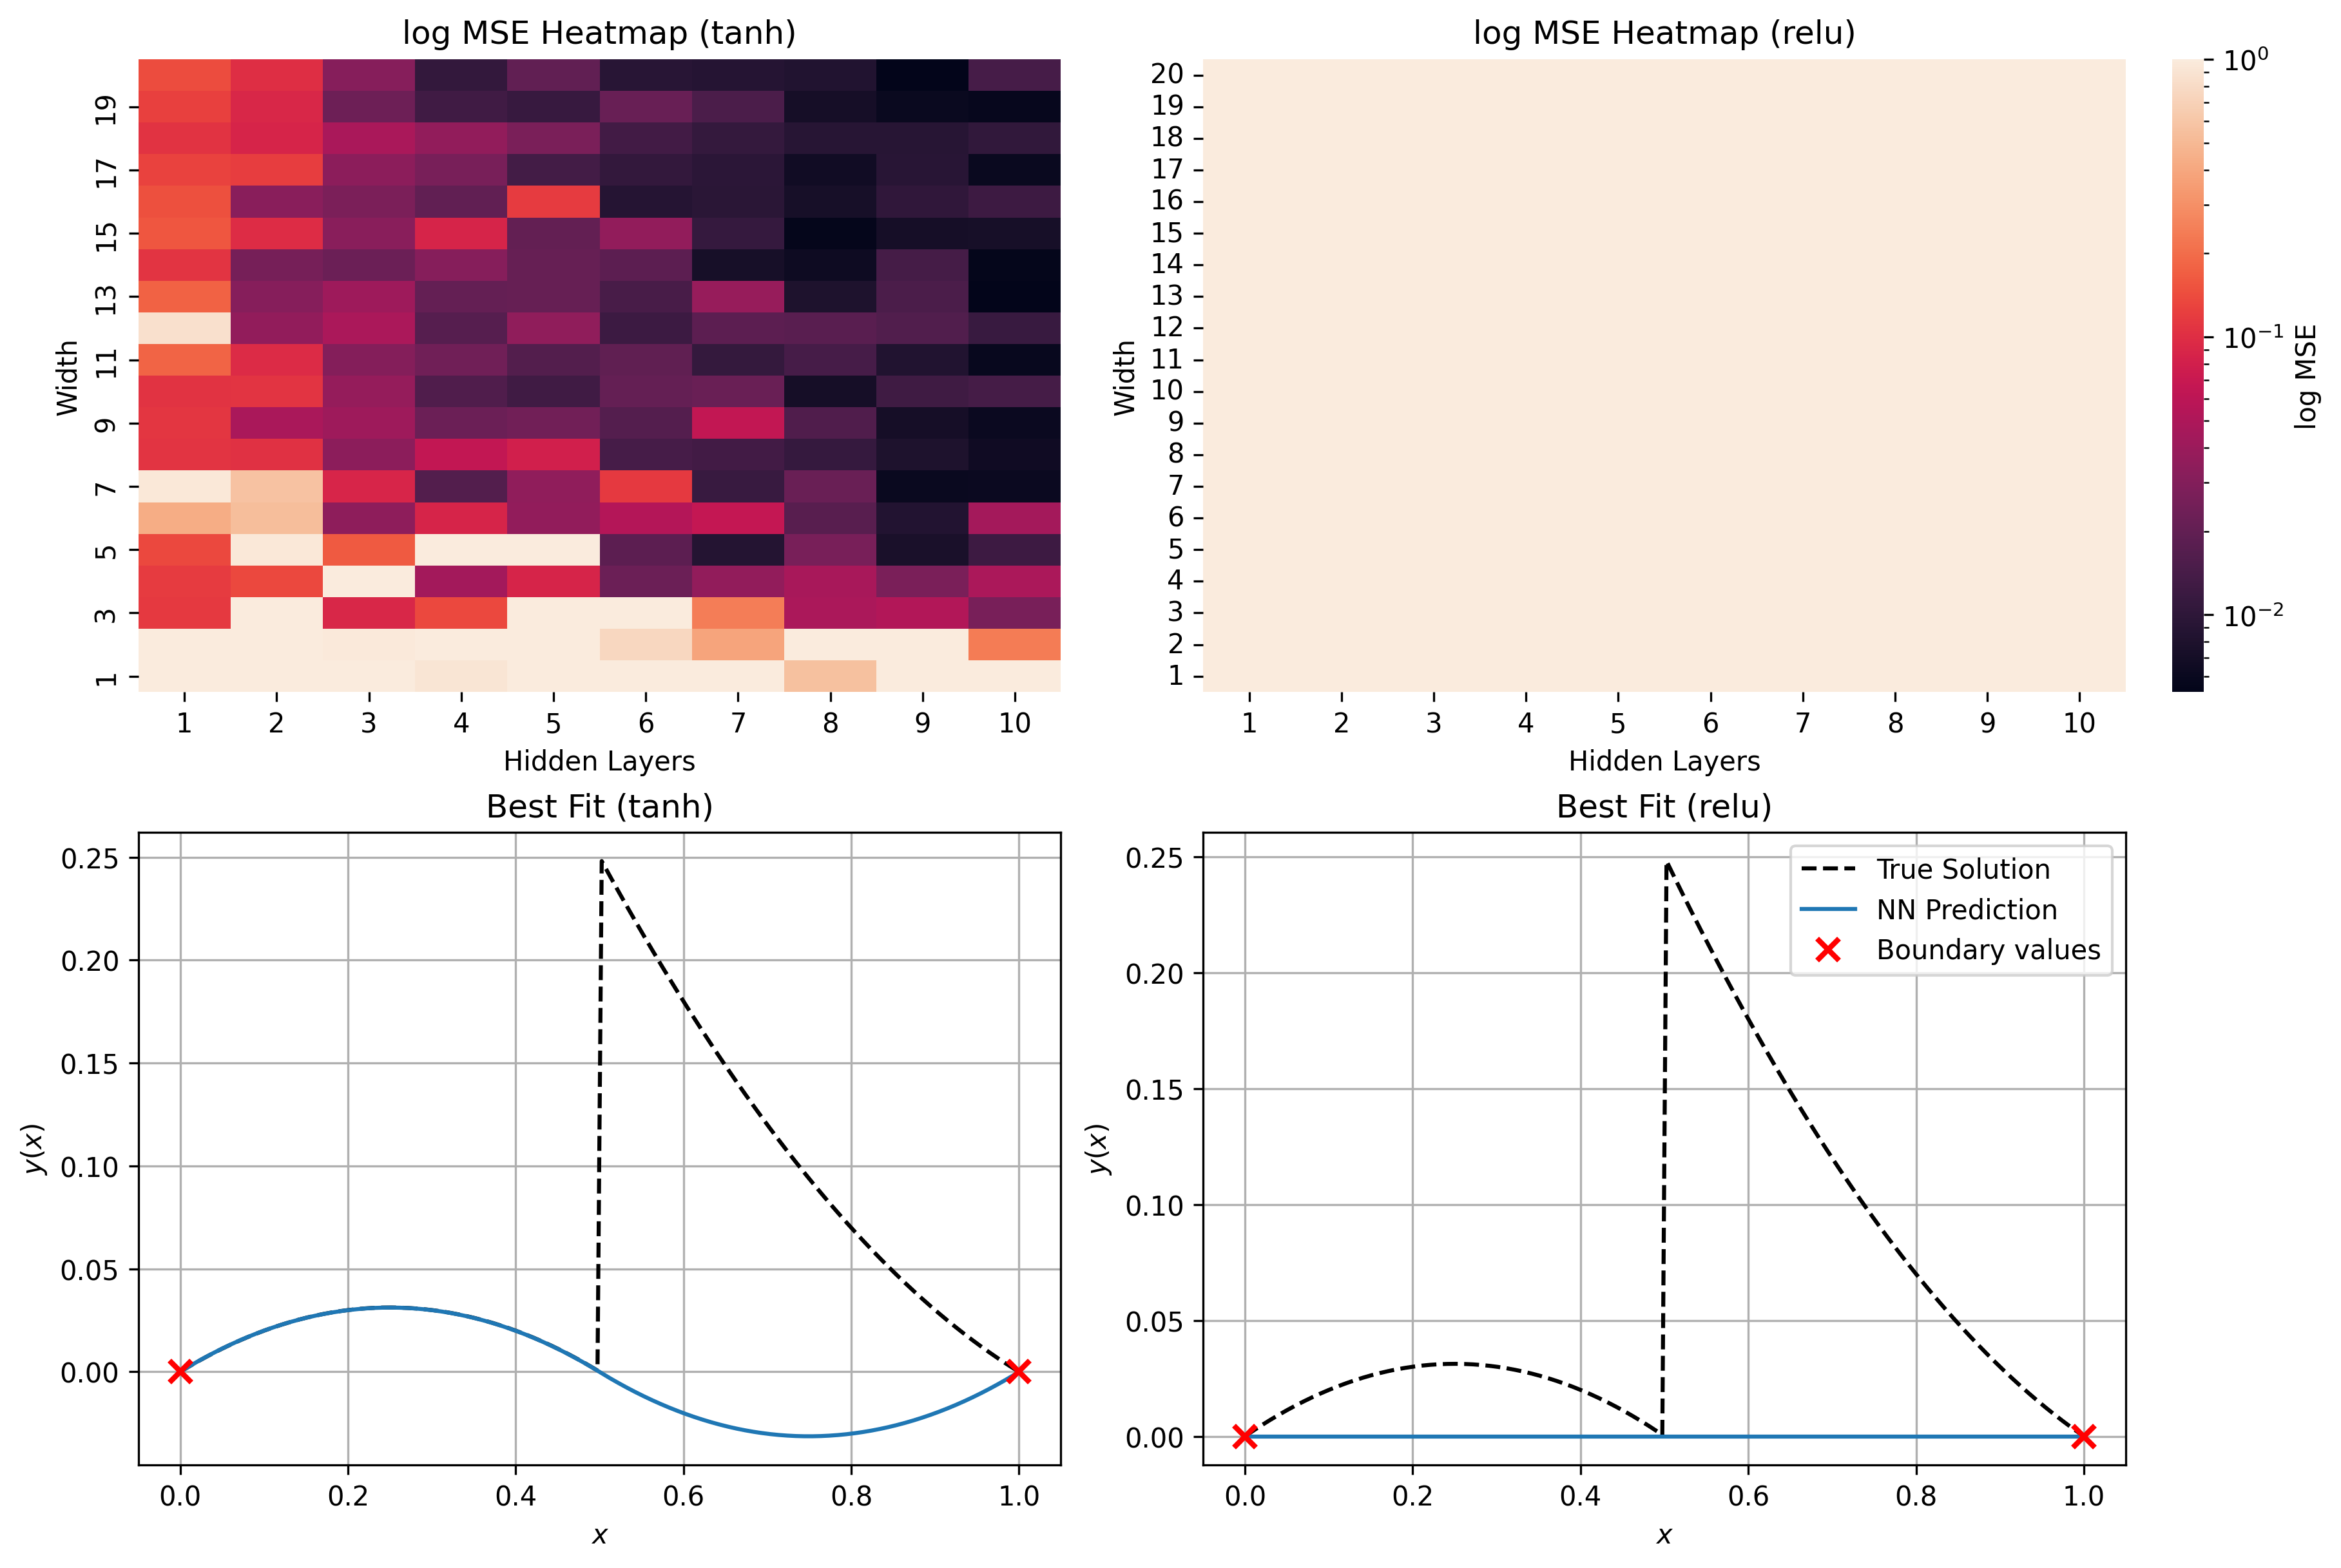
\includegraphics[width=\textwidth]{graphics/bvp_piecewise_combined.png}
    \caption{Comparison of architectural performance for the piecewise-forced BVP using two 
    activation functions. Each column shows the MSE heatmap (log scale) and best-fit solution.}
    \label{fig:bvp_piecewise_sidebyside}
\end{figure}

ReLU once again fails to capture the underlying structure of the solution, instead converging to a 
trivial fit that satisfies only the boundary conditions. In contrast, networks using the 
\(\tanh\) activation function show clear improvement with increased width and depth. 
Interestingly, rather than adapting to the discontinuity in the forcing term, the 
\(\tanh\) networks tend to converge toward smooth, sinusoidal-like approximations.

\section{Extension: Partial Differential Equations}\label{sec:pdes}
Having assessed neural network performance across a range of ordinary differential equation problems,
we now turn to a more challenging class: partial differential equations (PDEs). In this section, 
we consider a single representative elliptic PDE posed on a two-dimensional domain:
\[
\begin{aligned}
    -\nabla^2 u(x, y) &= f(x, y), \quad \text{for } (x, y) \in \Omega := (0,1)^2, \\
    u(x, y) &= 0, \quad \text{for } (x, y) \in \partial \Omega,
\end{aligned}
\]
where the forcing function is given by
\[
f(x, y) = 13\pi^2 \sin(2\pi x)\sin(3\pi y).
\]
This problem admits an exact solution \( u(x, y) = \sin(2\pi x)\sin(3\pi y) \), which is smooth, bounded, 
and vanishes on the boundary of the domain.

Our goal is to assess the ability of neural networks to recover this solution from collocation data 
sampled over the interior and boundary of the domain. Based on prior results, we restrict our 
attention to the \(\tanh\) and Swish activation functions, as ReLU has been shown to perform poorly 
in earlier experiments. We follow a similar methodology to that used in the ODE setting: 
systematically varying depth and width of the network and evaluating performance using mean 
squared error over a dense evaluation grid. We sample 1000 points internally and 200 points 
from the boundary, all points being equidistantly spaced.

In addition to architectural comparisons, we also investigate the robustness of the best-performing 
networks to data scarcity. Specifically, we assess how the approximation quality degrades as 
the number of training (collocation) points is reduced, thereby evaluating the sample efficiency 
of neural networks in recovering PDE solutions from limited information.

\subsection{Architectural Performance on the Poisson Problem}

 Figure~\ref{fig:pde_comparison} shows the results of our architectural analysis. We observe
consistent trends across both activation functions: increasing network width generally 
leads to improved accuracy, while depth plays a subtler role. The best models for both $\tanh$ and 
Swish achieve high-quality approximations to the true solution, closely matching the ground truth 
throughout most of the domain. However, the absolute error plots reveal that the Swish-based network 
produces a slightly more accurate fit overall, particularly along the domain boundaries. While both 
models perform well in the central region, the $\tanh$ network exhibits noticeable deviations near the 
edges, whereas the Swish model only shows small discrepancies at the corners. This suggests that the 
Swish activation may offer improved boundary adherence in this context, potentially due to its smooth 
yet non-saturating properties.

\begin{figure}[htbp]
    \centering
    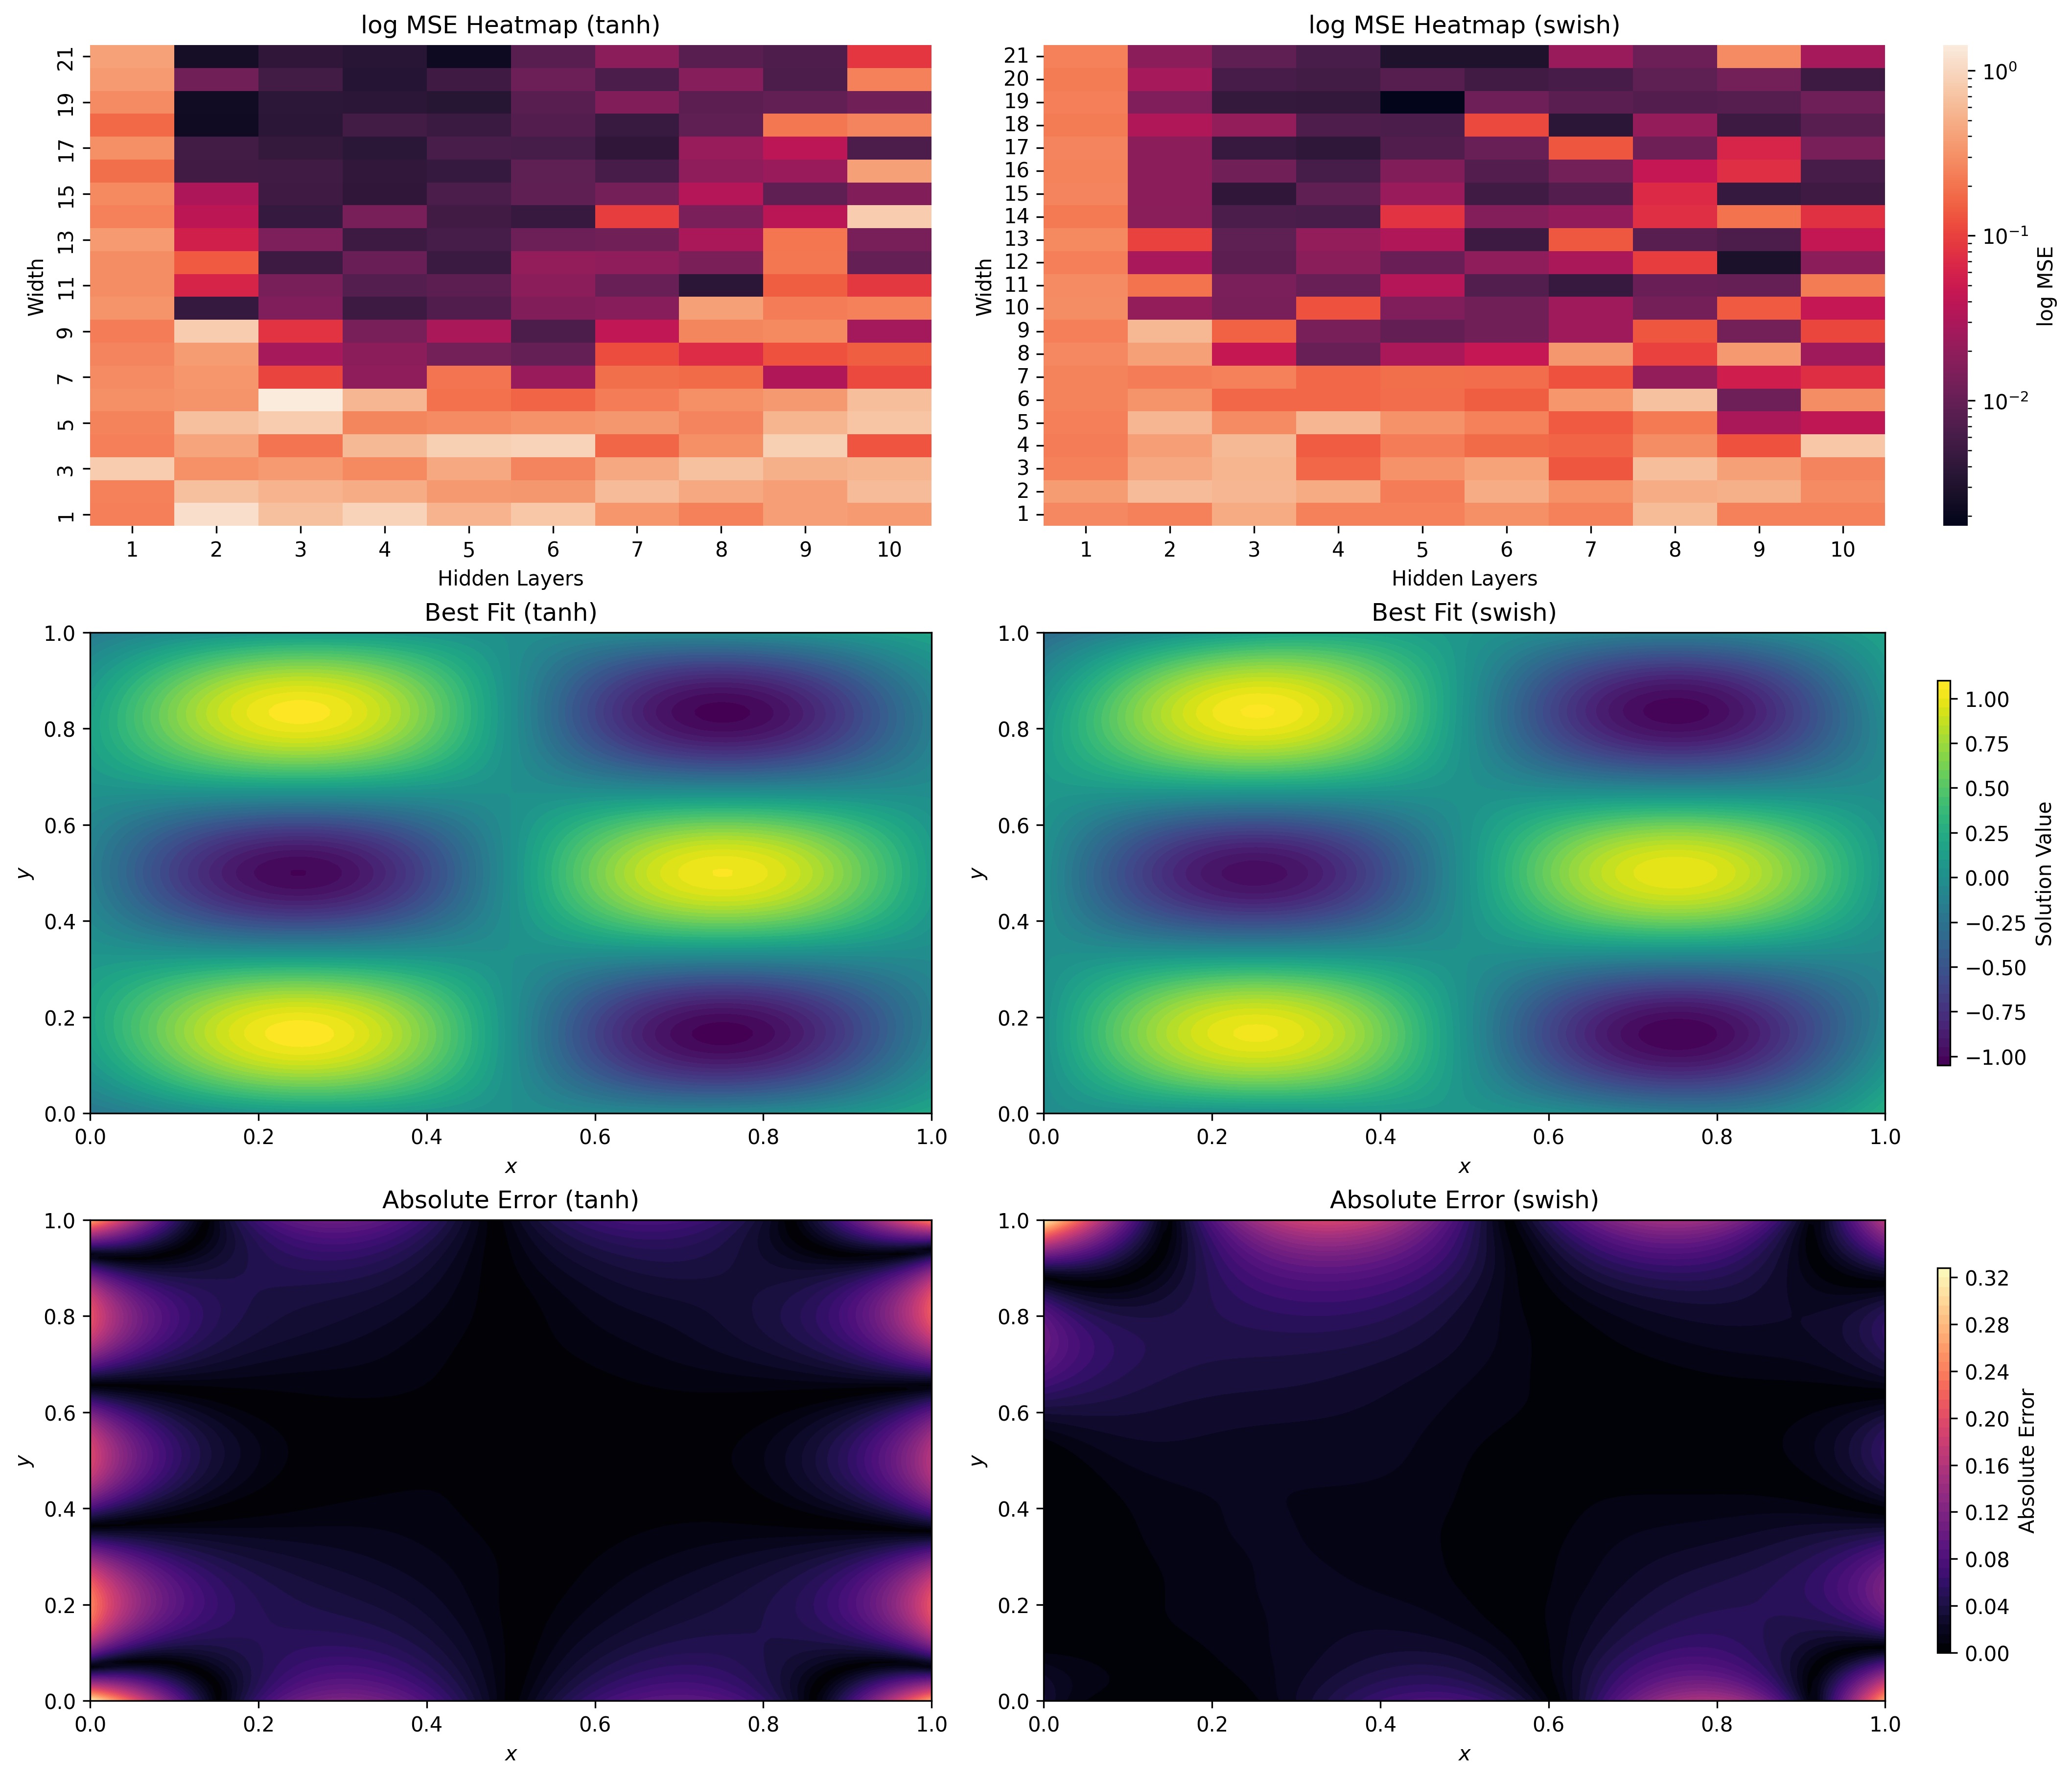
\includegraphics[width=0.9\textwidth]{graphics/pde_poisson_architecture_comparison.png}
    \caption{Comparison of neural network performance on the two-dimensional Poisson problem using the 
    $\tanh$ and Swish activation functions. Top row: log-scaled MSE heatmaps across architectural 
    configurations. Middle row: predicted solutions from the best-performing networks. Bottom row: 
    corresponding absolute error plots.}
    \label{fig:pde_comparison}
\end{figure}

We therefore elect to use the best-performing neural network from the above found, and now 
examine how this network performs as training points are reduced in the next section.

\subsection{Robustness to Reduced Training Data}

We now assess the sensitivity of neural network approximations to the number of training points, 
using the best-performing architecture from the preceding analysis. We vary the number of internal 
and boundary training points and illustrate the resulting accuracy in 
Figure~\ref{fig:training_point_comparison}.

\begin{figure}[t]
    \centering
    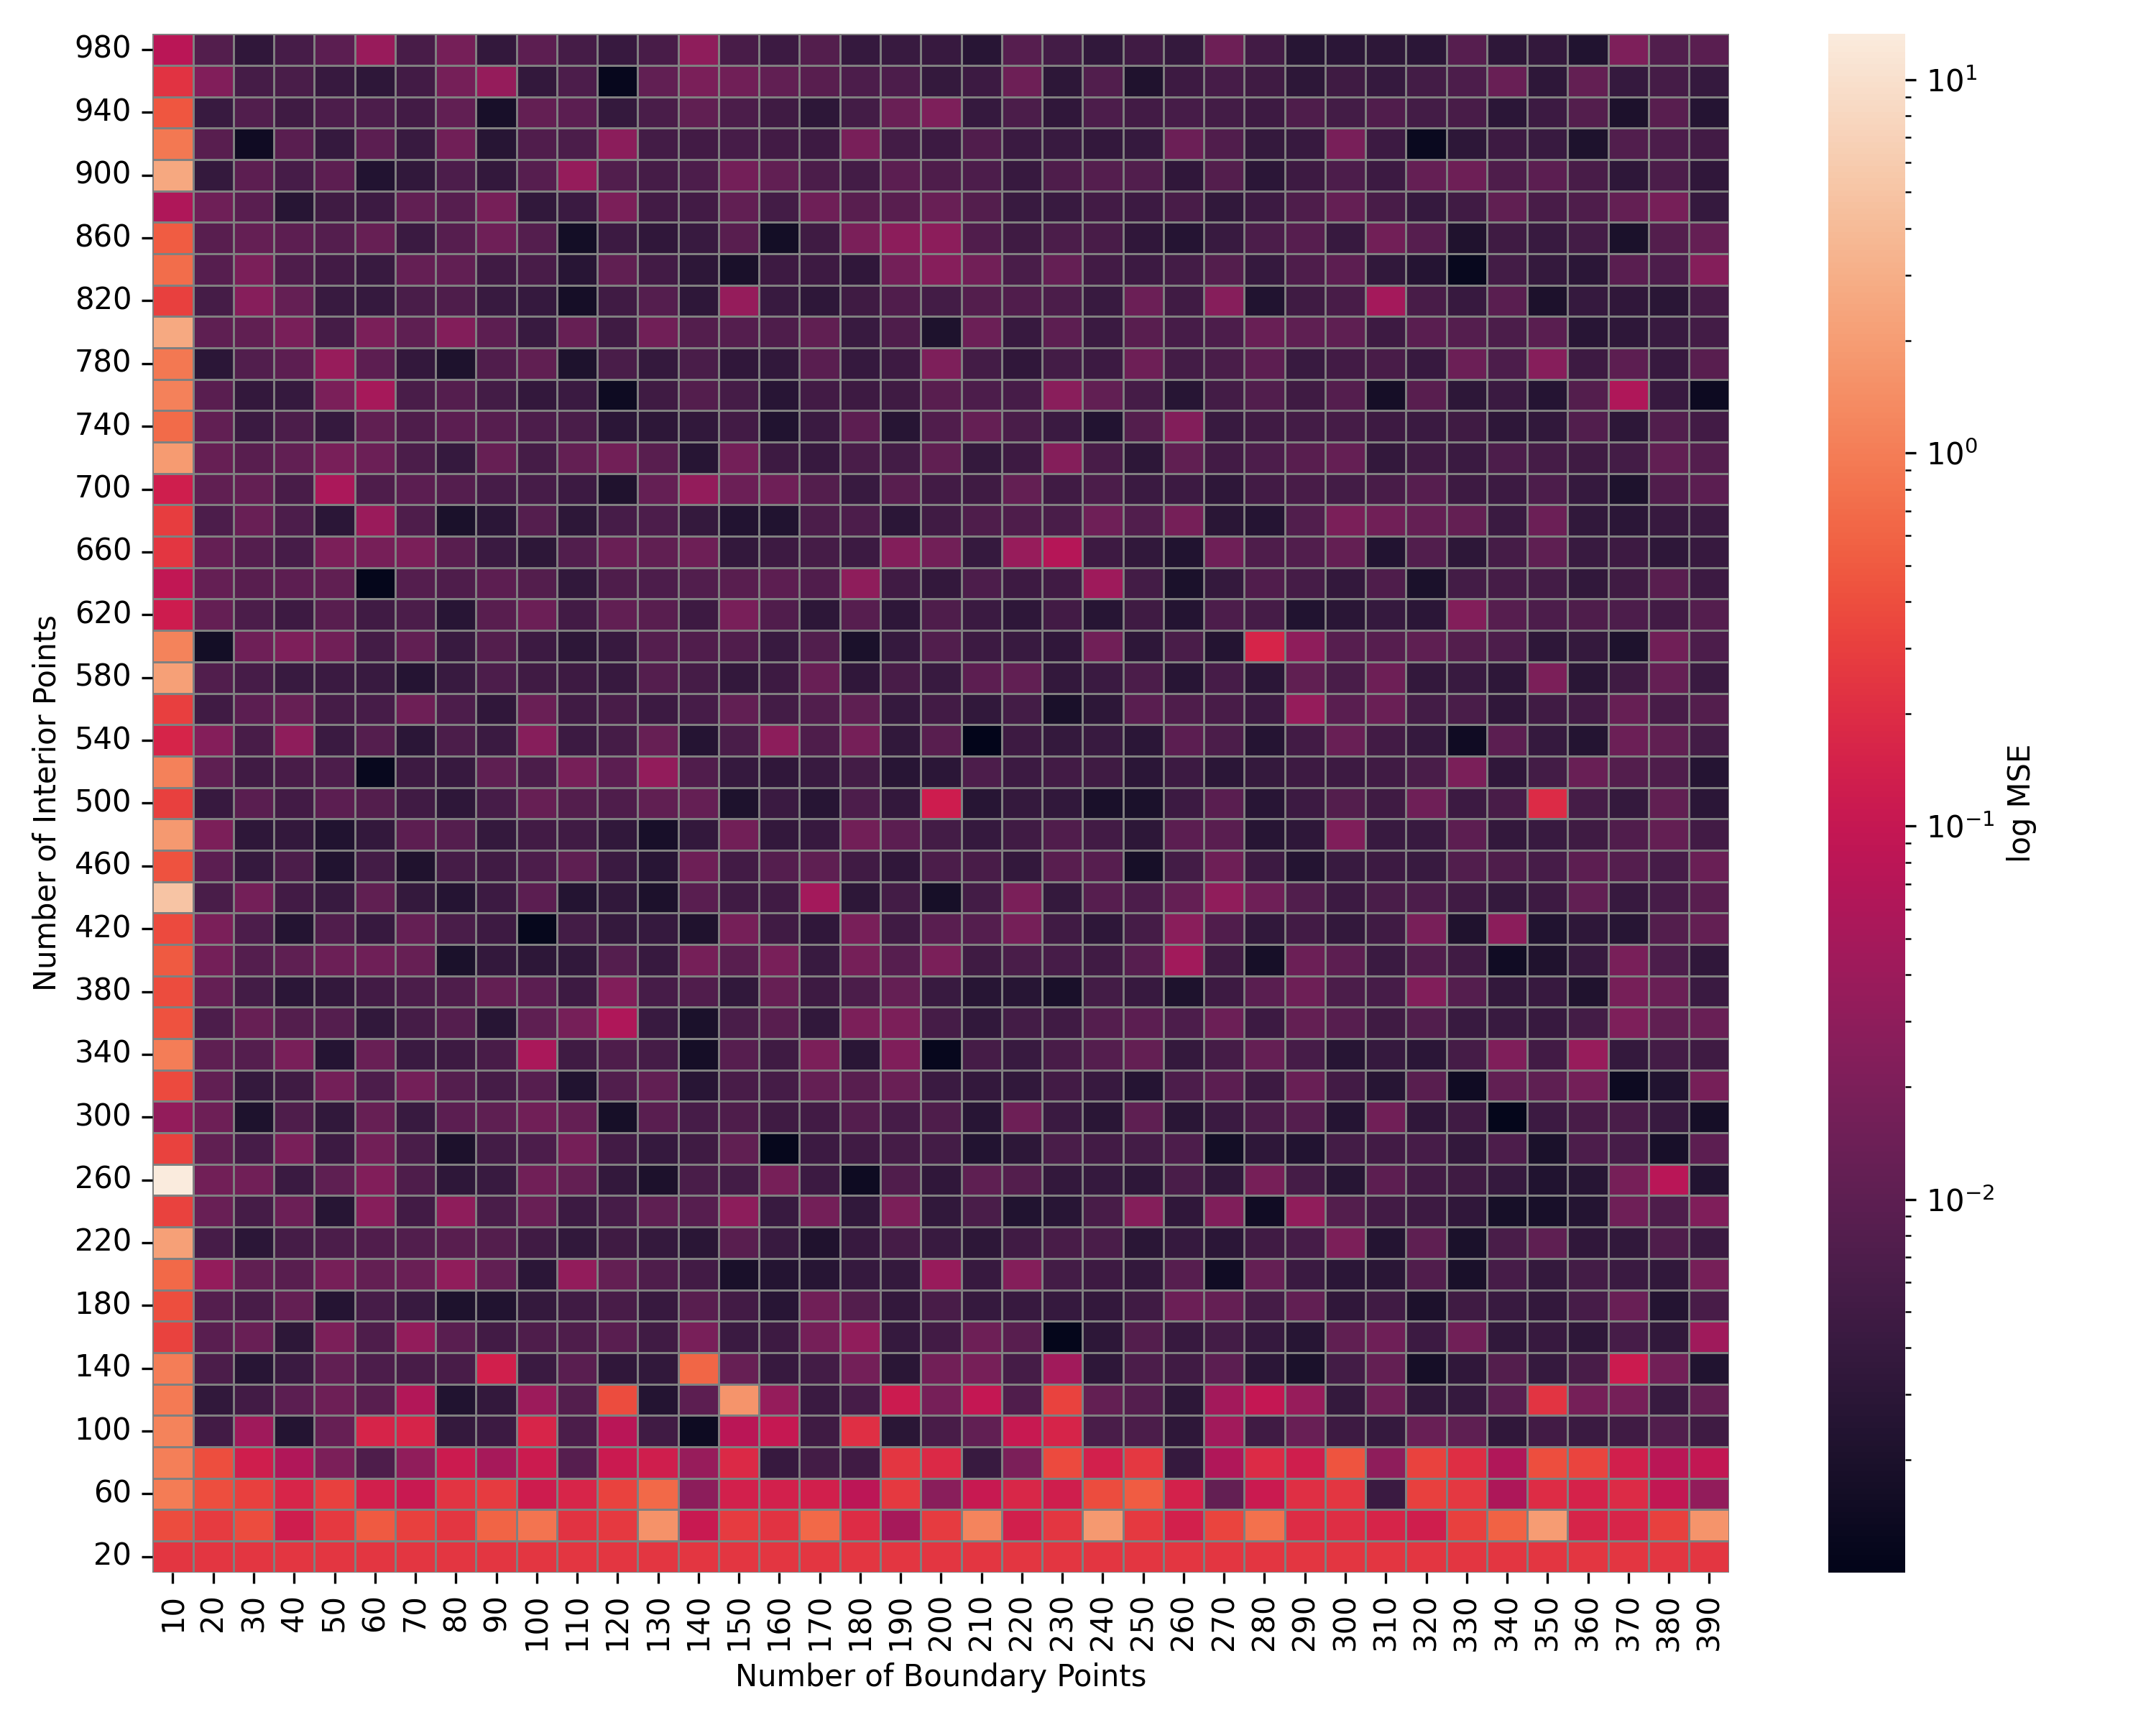
\includegraphics[width=0.75\textwidth]{graphics/pde_uniform_sampling_heatmap.png}
    \caption{Mean squared error heatmap showing how approximation accuracy varies with the number of internal and boundary training points.}
    \label{fig:training_point_comparison}
\end{figure}

The heatmap shows rapid convergence to high accuracy even with relatively sparse training points. 
Notably, performance improvements diminish significantly beyond approximately 100 internal points and
20 boundary points, indicating a clear threshold for obtaining an accurate solution. To better 
illustrate this threshold effect, Figure~\ref{fig:stacked_predictions} compares model predictions 
just below and at this threshold.

\begin{figure}[h]
    \centering
    \begin{subfigure}[t]{0.8\textwidth}
        \centering
        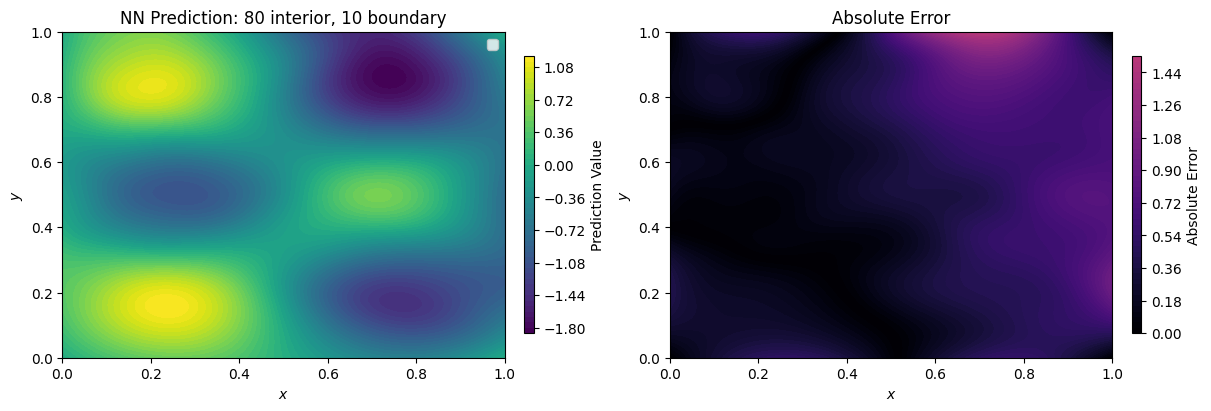
\includegraphics[width=\textwidth]{graphics/pde_points_80_10.png}
        \label{fig:prediction_80}
    \end{subfigure}
    
    \vspace{1em} 
    
    \begin{subfigure}[t]{0.8\textwidth}
        \centering
        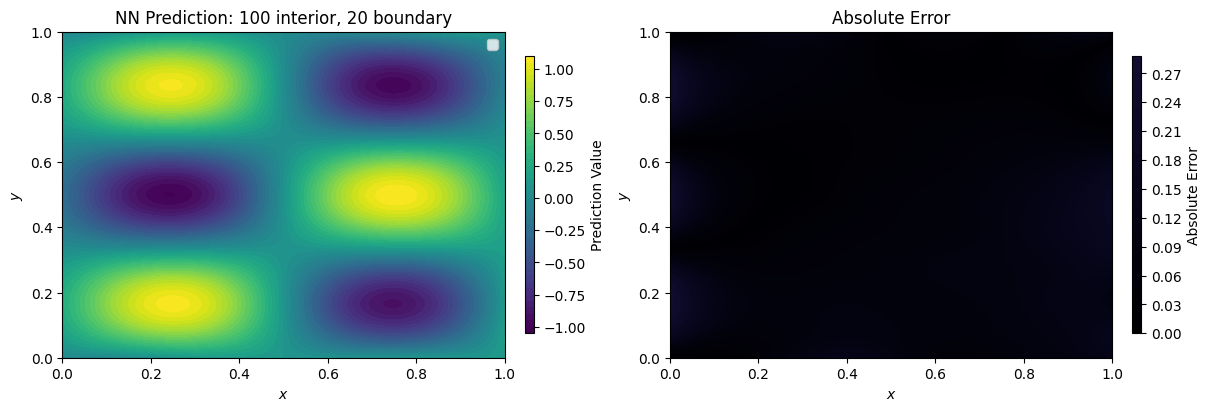
\includegraphics[width=\textwidth]{graphics/pde_points_100_20.png}
        \label{fig:prediction_100}
    \end{subfigure}
    \caption{Comparison of neural network predictions illustrating improved accuracy with moderate increases in training data.}
    \label{fig:stacked_predictions}
\end{figure}

Figure~\ref{fig:stacked_predictions} highlights how adding a modest number of training points 
substantially improves the accuracy and resolution of the neural network approximation. The 
prediction with 100 internal and 20 boundary points is notably sharper and exhibits significantly 
reduced error across the domain. The reported error in each case is computed as the mean squared 
error evaluated on 1000 equidistant points across the domain. These results confirm the robustness 
of neural network methods, achieving accurate PDE solutions with a relatively sparse distribution 
of training data.
\section{Conclusion}\label{sec:conclusion}

\printbibliography
\end{document}